\subsubsection{Strain rate and spin tensor} \label{ss:srst}
\index{general}{Velocity Gradient}
\index{general}{Strain Rate}
\index{general}{Spin Tensor}

The velocity gradient is given in Cartesian coordinates by:
\begin{equation}
\vec\nabla\vec\upnu = 
\left(
\begin{array}{ccc}
\frac{\partial u}{\partial x} & \frac{\partial v}{\partial x} & \frac{\partial w}{\partial x} \\\\
\frac{\partial u}{\partial y} & \frac{\partial v}{\partial y} & \frac{\partial w}{\partial y} \\\\
\frac{\partial u}{\partial z} & \frac{\partial v}{\partial z} & \frac{\partial w}{\partial z} 
\end{array}
\right)
\end{equation}
It can be decomposed into its symmetric and skew-symmetric parts according to:
\begin{equation}
\vec\nabla\vec\upnu = \vec\nabla^s\vec\upnu + \vec\nabla^w\vec\upnu = \dot{\bm \varepsilon}(\vec \upnu) +  \dot{\bm \omega}(\vec \upnu)
\end{equation}
The symmetric part is called the strain rate (or rate of deformation):
\begin{equation}
\dot{\bm \varepsilon}(\vec \upnu) = \frac{1}{2}\left( \vec\nabla\vec\upnu + (\vec\nabla\vec\upnu)^T \right)
\end{equation}
The skew-symmetric tensor is called spin tensor (or vorticity tensor):
\begin{equation}
\dot{\bm \omega}(\vec \upnu) = \frac{1}{2}\left( \vec\nabla\vec\upnu - (\vec\nabla\vec\upnu)^T \right)
\end{equation}

\begin{remark}
The velocity gradient tensor is sometimes denoted by ${\bm L}=\vec\nabla\vec\upnu$.
\end{remark}

\begin{remark}
In the mathematical literature a different notation for the strain rate tensor is often used, i.e. 
$D(\vec \upnu)$, such as for instance in Fullsack (1995) \cite{full95}.
\end{remark}

%.............................................
\subsection{Viscous Newtonian rheology}

The relationship between velocity-related stresses and
velocity derivatives is such that the total stress tensor has the form \cite{berc09}
\begin{equation}
{\bm \sigma} = -p {\bm 1} + {\bm A}:\dot{\bm \varepsilon}
\end{equation}
where $p$ is the thermodynamic pressure which is a function of the density $\rho$ and the temperature $T$ (an equation of state is then needed)
and ${\bm A}$ is the fourth-rank stiffness tensor.

Since both the stress and the strain tensors are symmetric and for isotropic 
fluids we have \cite{malvern}
\begin{equation}
{\bm A}:\dot{\bm \varepsilon} = \lambda (\vec\nabla\cdot\vec\upnu) {\bm 1} + 2\eta \dot{\bm \varepsilon}
\end{equation}
where $\lambda$ is the bulk viscosity and $\eta$ is the dynamic viscosity\footnote{also sometimes called shear viscosity}. 
The stress tensor is then 
\begin{equation}
{\bm \sigma} = (-p  + \lambda (\vec\nabla\cdot\vec\upnu)) {\bm 1} + 2\eta \dot{\bm \varepsilon}
\end{equation}
By writing 
\[
\dot{\bm \varepsilon} = \frac{1}{3}{\text tr}(\dot{\bm \varepsilon}) {\bm 1} + \dot{\bm \varepsilon}^d =
 \frac{1}{3}(\vec\nabla\cdot\vec\upnu) {\bm 1} + \dot{\bm \varepsilon}^d
\]
where $\dot{\bm \varepsilon}^d$ is the deviatoric strain rate tensor and 
(in Cartesian coordinates)
\begin{equation}
\vec\nabla\cdot\vec\upnu = 
\text{div} (\vec\upnu ) =
{\text tr}(\dot{\bm \varepsilon}) =
\frac{\partial u}{\partial x}+ 
\frac{\partial v}{\partial y}+ 
\frac{\partial w}{\partial z} 
\end{equation} 
where $\text{tr}$ is the trace operator, we arrive at
\begin{eqnarray}
{\bm \sigma} 
&=& (-p+\lambda(\vec\nabla\cdot\vec\upnu)) {\bm 1} + 2\eta \left[ \frac{1}{3}(\vec\nabla\cdot\vec\upnu) {\bm 1} + \dot{\bm \varepsilon}^d \right] \\
&=& \left[ -p+\left(\lambda+\frac{2}{3}\eta\right)(\vec\nabla\cdot\vec\upnu)\right] {\bm 1} + 2\eta  \dot{\bm \varepsilon}^d  
\end{eqnarray}
Introducing the second viscosity $\zeta=\lambda+\frac{2}{3}\eta$:
\begin{eqnarray}
{\bm \sigma} 
&=& \left[ -p+ \zeta (\vec\nabla\cdot\vec\upnu)\right] {\bm 1} + 2\eta  \dot{\bm \varepsilon}^d \\ 
&=&  -\overline{p} {\bm 1} + 2\eta  \dot{\bm \varepsilon}^d  
\end{eqnarray}
The effect of the volume viscosity $\zeta$ is that the mechanical pressure $\overline{p}$
is not equivalent to the thermodynamic pressure $p$ 
\begin{equation}
\overline{p}=p - \zeta (\vec\nabla\cdot\vec\upnu)
\end{equation}
In other words: the isotropic average of the total stress is {\sl not} the pressure term!
This difference is usually neglected (and it is safe to do so, see \cite[section 7.02.3.2.2]{berc09}) 
by explicitly assuming $\zeta=0$ (also called the Stokes assumption \cite[p256]{scto01}), 
so that one can then refer to pressure as a single well-defined value.
Note that in the case of an incompressible Newtonian Fluid, 
the strain rate tensor is deviatoric $({\text tr}(\dot{\bm \varepsilon}) = \text{div}(\vec\upnu) =0)$ and the above considerations vanish.

Finally, for both compressible and incompressible flow, the stress tensor becomes simply
\begin{mdframed}[backgroundcolor=blue!5]
\begin{equation}
{\bm \sigma}=-p {\bm 1} + 2\eta \dot{\bm \varepsilon}^d = -p {\bm 1} + {\bm \tau}
\end{equation}
\end{mdframed}
where ${\bm \tau} = 2\eta \dot{\bm \varepsilon}^d$ is the deviatoric stress tensor.

\begin{remark}
On page 256 of Schubert, Turcotte and Olson \cite{scto01}, equation 6.5.3, the authors write $\tau_{ii}/3=k_B e_{ii}$ while stating that $\tau$ is deviatoric in equation 6.4.2. 
This is an obvious conflict of notations. 
\end{remark}

%------------------------------------------------------------------------
\subsection{The heat transport equation - energy conservation equation \label{ss:hte}}

The heat contained within a volume $dV$ is $\rho C_p T dV$ where 
$C_p$ is the specific heat. The total heat ${\cal H}$ contained
by $V$ is the sum ( or integral) of all the elements within $V$:
\[
{\cal H}=\int_V \rho C_p T dV
\]
Changes in ${\cal H}$ can only occur if heat flows across the surface $S$. 
If $Q$ is the rate at which heat flows outward, then the rate of change of ${\cal H}$ 
must equal $Q$, or
\[
-\frac{\partial {\cal H}}{\partial t} = Q
\]
The negative sign is required because the volume cools if $Q$ is positive. 
The heat flux depends on the temperature gradient $\vec\nabla T$ , 
and heat always flows down the temperature gradient. Hence the heat
flux across the surface element $dS$, $dQ$, is
\[
dQ= - k \vec\nabla T \cdot \vec{n} \; dS
\]
where $k$ is the thermal conductivity. The dot product between $\vec\nabla T$ and $\vec{n}dS$ 
takes the direction of the temperature gradient into account.
We can then write:
\[
-\frac{\partial }{\partial t} \int_V \rho C_p T dV = - \int_S  k \vec\nabla T \cdot \vec{n} \; dS
\]
Using Gauss' theorem th right hand side becomes:
\[
\int_S  k \vec\nabla T \cdot \vec{n} \; dS
= 
\int_V \vec\nabla \cdot ( k \vec\nabla T \cdot ) dV
\]
so that:
\[
\int_V \left[ \frac{\partial }{\partial t} (\rho C_p T) - \vec\nabla \cdot( k \vec\nabla T ) \right] dV 
\]
Since $V$ can be any volume enclosed by an arbitrary surface, this 
equation can only be true if the term in square brackets is zero everywhere, or:
\[
\rho C_p \frac{\partial T}{\partial t}  =  \vec\nabla \cdot( k \vec\nabla T ) 
\]
assuming density and specific heat to be constant in time.
In a fluid which moves, the heat transport must include a term
\[
\int_S \rho C_p T \vec\upnu\cdot \vec{n} \; dS
\]
to take account of the heat carried by the fluid moving with velocity $\vec\upnu$. 
This term is called the advection term in the equations, and we then have:
\[
\rho C_p \left( 
\frac{\partial T}{\partial t} + (\vec\upnu \cdot \vec\nabla) T \right) =  \vec\nabla \cdot( k \vec\nabla T ) 
\]

\todo[inline]{join what is above to what comes after this}


Let us start from the heat transport equation as shown in Schubert, Turcotte and Olson \cite{scto01}:
\begin{equation}
\rho C_p \frac{DT}{Dt} - \alpha T \frac{Dp}{Dt} = {\vec \nabla} \cdot k {\vec \nabla} T + \Phi + \rho H  
\end{equation}
with $D/Dt$ being the total derivatives, i.e. 
\begin{equation}
\frac{DT}{Dt} = \frac{\partial T}{\partial t} + {\vec \upnu}\cdot {\vec \nabla}T
\qquad
\text{and}
\qquad
\frac{Dp}{Dt} = \frac{\partial p}{\partial t} + {\vec \upnu}\cdot {\vec \nabla}p
\end{equation}
Solving for temperature, this equation is often rewritten as follows:
\begin{mdframed}[backgroundcolor=blue!5]
\begin{equation}
\rho C_p \frac{DT}{Dt} - {\vec \nabla} \cdot k {\vec \nabla} T =  \alpha T \frac{Dp}{Dt} + \Phi + \rho H  
\end{equation}
\end{mdframed}
where $\Phi$ is the shear heating \cite[p287]{reddybook2}. In many publications, $\Phi$ 
is given by $\Phi=\tau_{ij}\partial_j \upnu_i={\bm \tau}:{\vec \nabla}{\vec \upnu}$.

In what follows I use the index notation as it makes for easier derivations:
\begin{eqnarray}
\Phi 
&=& \tau_{ij}\partial_j \upnu_i \nonumber\\
&=& 2 \eta \dot{\varepsilon}_{ij}^d\partial_j \upnu_i \nonumber\\
&=& 2 \eta \frac{1}{2}\left( \dot{\varepsilon}_{ij}^d\partial_j \upnu_i + \dot{\varepsilon}_{ji}^d\partial_i u_j \right) \nonumber\\
&=& 2 \eta \frac{1}{2}\left( \dot{\varepsilon}_{ij}^d\partial_j \upnu_i + \dot{\varepsilon}_{ij}^d\partial_i u_j \right) \nonumber\\
&=& 2 \eta  \dot{\varepsilon}_{ij}^d  \frac{1}{2}\left(\partial_j \upnu_i + \partial_i u_j \right) \nonumber\\
&=& 2 \eta  \dot{\varepsilon}_{ij}^d   \dot{\varepsilon}_{ij} \nonumber\\
&=& 2 \eta  \dot{\bm \varepsilon}^d :  \dot{\bm \varepsilon} \nonumber\\
&=& 2 \eta  \dot{\bm \varepsilon}^d : \left( \dot{\bm \varepsilon}^d +\frac{1}{3} ({\vec \nabla}\cdot{\vec \upnu}) {\bm 1} \right)\nonumber\\
&=& 2 \eta  \dot{\bm \varepsilon}^d : \dot{\bm \varepsilon}^d 
+ 2 \eta  \dot{\bm \varepsilon}^d : {\bm 1} ({\vec \nabla}\cdot{\vec \upnu}) \nonumber\\ 
&=& 2 \eta  \dot{\bm \varepsilon}^d : \dot{\bm \varepsilon}^d 
\end{eqnarray}
Finally
\begin{equation}
\Phi = {\bm \tau}:{\vec \nabla}{\vec \upnu} = 2 \eta  \dot{\bm \varepsilon}^d : \dot{\bm \varepsilon}^d
= 2 \eta \left( (\dot{\varepsilon}_{xx}^d)^2 + (\dot{\varepsilon}_{yy}^d)^2 + 2(\dot{\varepsilon}_{xy}^d)^2 \right)
\end{equation}

\paragraph{Non-dimensionalisation}
We can scale the equations as follows:
\[
T =T_0 T'
\qquad 
t =\frac{a^2}{\kappa \; Ra} t'
\qquad
\vec\upnu = \frac{\kappa \; Ra}{a} \vec\upnu'
\]
where $a$ is a characteristic length, giving:
\[
Ra \left( \frac{\partial T'}{\partial t'}  + \vec\upnu'\cdot\vec\nabla' T' \right)
=\Delta' T'
\]
$Ra$ is is the only parameter which affects the convection. When it becomes very large 
this equation essentially becomes an advection equation. 





%------------------------------------------------------------------------
\subsection{The momentum conservation equations} 

Because the Prandlt number is virtually zero in Earth science applications the Navier-Stokes 
equations reduce to the Stokes equation:
\begin{equation}
{\vec \nabla}\cdot {\bm \sigma} + \rho {\vec g} = \vec{0}
\end{equation}
Since 
\begin{equation}
{\bm \sigma} = -p {\bm 1} + {\bm \tau}
\end{equation}
it also writes
\begin{equation}
-{\vec \nabla}p + {\vec \nabla}\cdot {\bm \tau} + \rho {\vec g} = \vec{0}
\end{equation}
Using the relationship ${\bm \tau} = 2 \eta \dot{\bm \varepsilon}^d$ we arrive at 
\begin{mdframed}[backgroundcolor=blue!5]
\begin{equation}
-{\vec \nabla}p + {\vec \nabla}\cdot (2 \eta \dot{\bm \varepsilon}^d ) + \rho {\vec g} = \vec{0}
\end{equation}
\end{mdframed}

%------------------------------------------------------------------------
\subsection{The mass conservation equations} 
\index{general}{Solenoidal Field} 
\index{general}{Divergence-free}
\index{general}{Continuity Equation}
\index{general}{Mass Conservation Equation}

The mass conservation equation (often called continuity equation) is given by
\[
\frac{D\rho}{Dt} + \rho {\vec \nabla}\cdot{\vec \upnu} = 0
\]
or, since 
\[
\frac{D\rho}{Dt} = \frac{\partial \rho}{\partial t} + {\vec \upnu}\cdot {\vec \nabla}\rho
\]
then 
\[
\frac{D\rho}{Dt} + \rho {\vec \nabla}\cdot{\vec \upnu} = 
\frac{\partial \rho}{\partial t} + {\vec \upnu}\cdot {\vec \nabla}\rho
 + \rho {\vec \nabla}\cdot{\vec \upnu} = 0 
\]
and finally:
\begin{mdframed}[backgroundcolor=blue!5]
\[
\frac{\partial \rho}{\partial t} + {\vec \nabla}\cdot(\rho {\vec \upnu}) = 0
\]
\end{mdframed}
In the case of an incompressible flow, then $\partial \rho/\partial t=0$ and 
${\vec \nabla}\rho=0$, i.e. $D\rho/Dt=0$ and the remaining equation is simply:
\[
{\vec \nabla}\cdot{\vec \upnu} = 0
\]
A vector field that is divergence-free is also called 
solenoidal\footnote{\url{https://en.wikipedia.org/wiki/Solenoidal_vector_field}}.


In cylindrical coordinates $(r,\theta,\phi)$ 
the continuity equation for an incompressible fluid is :

\begin{mdframed}[backgroundcolor=blue!5]
\[
\frac{1}{r} \frac{\partial}{\partial r} (r \upnu_r) 
+
\frac{1}{r} \frac{\partial \upnu_\theta}{\partial \theta}
+
\frac{\partial \upnu_z}{\partial z}=0
\]
\end{mdframed}
\index{general}{Mass Conservation Equation (Cylindrical Coordinates)}


In spherical coordinates $(r,\theta,\phi)$ 
the continuity equation for an incompressible fluid is :

\begin{mdframed}[backgroundcolor=blue!5]
\[
\frac{1}{r^2} \frac{\partial}{\partial r} (r^2 \upnu_r) 
+
\frac{1}{r \sin\theta} \frac{\partial}{\partial \theta} (\upnu_\theta \sin\theta)
+
\frac{1}{r \sin\theta} \frac{\partial \upnu_\phi}{\partial \phi}=0
\]
\end{mdframed}
\index{general}{Mass Conservation Equation (Spherical Coordinates)}



%------------------------------------------------------------------------------
\subsection{The equations in ASPECT manual}
The following is lifted off the ASPECT manual.
We focus on the system of equations in a $d=2$- or $d=3$-dimensional
domain $\Omega$ that describes the motion of a highly viscous fluid driven
by differences in the gravitational force due to a density that depends on
the temperature. In the following, we largely follow the exposition of this
material in Schubert, Turcotte and Olson \cite{scto01}.

Specifically, we consider the following set of equations for velocity $\mathbf
u$, pressure $p$ and temperature $T$:
\begin{align}
  \label{eq:stokes-1}
  -\vec\nabla \cdot \left[2\eta \left(\dot{\bm \varepsilon}(\vec \upnu)
                                  - \frac{1}{3}(\vec\nabla \cdot \vec \upnu)\mathbf 1\right)
                \right] + \vec\nabla p &=
  \rho \vec g
  &
  & \textrm{in $\Omega$},
  \\
  \label{eq:stokes-2}
  \vec\nabla \cdot (\rho \vec v) &= 0
  &
  & \textrm{in $\Omega$},
  \\
  \label{eq:temperature}
  \rho C_p \left(\frac{\partial T}{\partial t} + \vec \upnu\cdot\vec\nabla T\right)
  - \vec\nabla\cdot k\vec\nabla T
  &=
  \rho H
  \notag
  \\
  &\quad
  +
  2\eta
  \left(\dot\varepsilon(\bm v) - \frac{1}{3}(\vec\nabla \cdot \vec \upnu)\mathbf 1\right)
  :
  \left(\dot\varepsilon(\bm v) - \frac{1}{3}(\vec\nabla \cdot \vec \upnu)\mathbf 1\right)
  \\
  &\quad
  +\alpha T \left( \bm v \cdot \vec\nabla p \right)
  \notag
  \\
  &\quad
  &
  & \textrm{in $\Omega$},
  \notag
\end{align}
where $\dot{\bm \varepsilon}(\vec\upnu) = \frac{1}{2}(\vec\nabla \vec\upnu + \vec\nabla \vec\upnu^T)$ is the symmetric gradient of the velocity (often called the
\textit{strain rate}).%

In this set of equations, \eqref{eq:stokes-1} and \eqref{eq:stokes-2}
represent the compressible Stokes equations in which $\mathbf v=\mathbf
v(\mathbf x,t)$ is the velocity field and $p=p(\mathbf x,t)$ the pressure
field. Both fields depend on space $\mathbf x$ and time $t$. Fluid flow is
driven by the gravity force that acts on the fluid and that is proportional to
both the density of the fluid and the strength of the gravitational pull.

Coupled to this Stokes system is equation \eqref{eq:temperature} for the
temperature field $T=T(\mathbf x,t)$ that contains heat conduction terms as
well as advection with the flow velocity $\mathbf v$. The right hand side
terms of this equation correspond to
\begin{itemize}
\item internal heat production for example due to radioactive decay;
\item friction (shear) heating;
\item adiabatic compression of material;
\end{itemize}

In order to arrive at the set of equations that ASPECT solves, 
we need to 
\begin{itemize}
\item neglect the $\partial p/\partial t$
\item neglect the $\partial \rho / \partial t$ 
\end{itemize}
from equations above. A partial answer is given in the next section. 

----------------------------------------

Also, their definition of the shear heating term $\Phi$ is:
\[
\Phi = k_B ({\bm \nabla}\cdot{\bm v})^2 + 2\eta \dot{\bm \varepsilon}^d:\dot{\bm \varepsilon}^d
\]
For many fluids the bulk viscosity $k_B$ is very small and is often taken to be zero, an assumption known
as the Stokes assumption: $k_B=\lambda+2\eta/3=0$. \index{general}{Bulk Viscosity}
Note that $\eta$ is the dynamic viscosity and $\lambda$ the second viscosity. 
\index{general}{Dynamic Viscosity}
\index{general}{Second Viscosity}
Also, 
\[
{\bm \tau}=2\eta \dot{\bm \varepsilon} + \lambda ({\bm \nabla}\cdot{\bm v}) {\bm 1}
\]
but since $k_B=\lambda+2\eta/3=0$, then $\lambda=-2\eta/3$ so 
\[
{\bm \tau}=2\eta \dot{\bm \varepsilon} -\frac{2}{3}\eta ({\bm \nabla}\cdot{\bm v}) {\bm 1} = 2\eta \dot{\bm \varepsilon}^d
\]

%---------------------------------------------------------------------------------------------------
\subsection{Equations for thermal convection in an anelastic, compressible, self-gravitating spherical mantle }
%------------------------------------------------------------------------------

What follows is borrowed from Section 2.1 of Gli{\v{s}}ovi{\'c} et al (2012) \cite{glfm12}.
We start from the conservation mass, momentum and energy equations (the full Navier-Stokes equations):
\begin{eqnarray}
\frac{\partial \rho}{\partial t} + \vec\nabla \cdot (\rho \vec\upnu) = \vec{0} \\
\rho \frac{D\vec\upnu}{Dt} = \vec\nabla\cdot {\bm \sigma} \\
\rho C_p \frac{D T}{Dt} = \vec\nabla \cdot k \vec\nabla T + \alpha T \frac{Dp}{Dt} + \Phi + Q
\end{eqnarray}
In solving for the mantle flow field that satisfies the equation of momentum conservation, 
we incorporate all effects arising from
self-gravitation and we must therefore explicitly consider the 3-D variation of 
gravity throughout Earth’s interior. The
gravitational acceleration is written as
\[
\vec{g} = \vec\nabla \phi
\]
where $\phi$ is Earth’s gravitational potential which satisfies Poisson's equation
\[
\Delta \phi = - 4 \pi {\cal G} \rho
\]
The gravitational potential is expressed as
\[
\phi = \phi_0(r) + \phi_1(r,\theta,\phi)
\]
where the subscript $0$ denotes a hydrostatic reference state, 
in which the structure of the mantle (density, gravity, pressure, temperature) varies
with radius alone and the subscript $1$ denotes all 3D perturbations arising from the 
thermal convection process. This decomposition makes sense in the context of a perfect sphere.

The total perturbed density and pressure fields in the mantle may similarly be expressed as
\[
\rho = \rho_0(r) + \rho_1(r,\theta,\phi)
\]
\[
p = p_0(r) + p_1(r,\theta,\phi)
\]
The equation of state relates the density perturbations to the temperature and pressure perturbations 
as follows
\[
\rho_1 = \rho_0[1-\alpha(T-T_0(r))+K^{-1} (p-p_0(r))] 
\]
where $K$ is the bulk modulus and the term $T_0(r)$ represents the horizontally averaged temperature (i.e.
the geotherm) which varies with radius only. The effects of compressibility on the density are found to be at least two orders of magnitude
smaller than the effects of temperature variations. Therefore, the last term 
of this equation is often neglected.

\index{general}{ALA}
\index{general}{Anelastic Liquid Approximation}
Important simplifications are made assuming the anelastic-liquid approximation 
(e.g. \cite{jamc80} Jarvis \& McKenzie (1980) \cite{jamc80},Solheim \& Peltier (1990) \cite{sope90}).
This approximation is justified because the velocities associated with mantle convection 
are very slow compared to the local sound speed and
hence acoustic waves cannot be generated by the slow changes in the mantle pressure field. 
We therefore neglect the time derivative of density, thereby eliminating sound waves:
\[
\frac{\partial \rho}{\partial t} \simeq 0
\] 
For the same reason, the pressure distribution may be considered (to first-order accuracy) 
as the pressure of a fluid in hydrostatic equilibrium which yields
\[
\frac{Dp}{Dt} = \frac{\partial p}{\partial t} + \vec\upnu\cdot\vec\nabla p 
\simeq
- u_r \rho_0(r) g_0(r)
\]
The equations are then rewritten in terms of dimensionless variables according to the relations:
\begin{eqnarray}
r'&=&\frac{r}{d} \\
\upnu' &=& \frac{\upnu}{U} \\
t' &=& \frac{U}{d/t} \\
T' &=& \frac{T}{\Delta T} \\
\rho' &=& \frac{\rho}{\rho_{0s}} \\
g' &=& \frac{g}{g_{0s}} \\
\phi' &=& \frac{\phi}{g_{0s}d} \\
\alpha' &=& \frac{\alpha}{\alpha_s} \\
p' &=& \frac{p}{\alpha_s \Delta T \rho_{0s} g_{0s} d} \\
\tau_{ij} &=& \frac{\tau_{ij}}{\alpha_s \Delta T \rho_{0s} g_{0s} d} \\
\eta' &=& \frac{\eta}{\eta_s} \\
k' &=& \frac{k}{k_s} \\
Q' &=& \frac{Q d^2}{k_s \Delta T} \\
U &=& \frac{\rho_{0s}g_{0s}\alpha_s \Delta T d^2}{\eta_s}
\end{eqnarray}

in which the primes represent the dimensionless variables, the subscript $s$ means 
that we consider the surface value of the variable to which it
is applied. The length scale $d$ and temperature scale $\Delta T$ are respectively 
the depth of the mantle and the difference of temperature between
the bottom and the top of the mantle. 

Often one deals with dimensionless variables and the primes
are dropped for notational convenience (this is the case in what follows).

It is a tedious but trivial exercise to show that the dimensionless equation of 
conservation of momentum is then written as follows:
\[
\rho \frac{Ra_s}{Pr_s} \frac{D\vec\upnu}{Dt} =
\frac{\rho}{\alpha_s \Delta T} \vec\nabla \phi - \vec\nabla p + \vec\nabla \cdot {\bm \tau}
\]
in which we introduce the surface Rayleigh $Ra_s$ and Prandtl $Pr_s$ numbers defined, 
respectively, by
\[
Ra_s=\frac{\rho_{0s}^2 C_p g_{0s} \alpha_s \Delta T d^3}{k_s \eta_s}
\qquad
\qquad
Pr_s= \frac{\eta_s C_p}{k_s}
\]
Because of the very high viscosity of mantle rocks, the left-hand term 
is smaller than the other terms by several orders of magnitude
and may therefore be neglected. This important simplification is called the 
infinite Prandtl number approximation. \index{general}{Prandtl number}

The equation of energy conservation may also be rewritten in terms of the surface Rayleigh number, as follows
\[
\frac{D T}{D t} = \frac{1}{\rho Ra_s} \left( \vec\nabla\cdot k\vec\nabla T + Q \right) 
+\frac{Di}{\rho} \left( -\alpha T \frac{Dp}{Dt} + \Phi  \right)
\]
where $Di$ is the dissipation number (see Peltier (1972) \cite{pelt72}) 
which measures the importance of compression work and frictional heating, and it is defined
as \index{general}{Dissipation Number}
\[
Di=\frac{\alpha_s g_{0s} d}{C_p}
\]
$Di$ also measures the ratio of the depth of mantle convection ($d$) to 
the adiabatic scale height ($C_p/\alpha g_0$ ) and for whole-mantle convection is
close to order 1 (see Jarvis \& McKenzie (1980) \cite{jamc80}).

After simplifications, the dimensionless system of governing equations is written as

\begin{eqnarray}
\vec\nabla\cdot(\rho_0 \vec\upnu) =0 \\
\frac{\rho}{\alpha_s \Delta T} \vec\nabla \phi - \vec\nabla p + \vec\nabla \cdot {\bm \tau} = \vec{0} \\
\frac{\partial T}{\partial t} + \vec\upnu\cdot\vec\nabla T =  
\frac{1}{\rho_0 Ra_s} \left( \vec\nabla\cdot k\vec\nabla T + Q \right) +
\frac{Di}{\rho_0} (-\alpha T \rho_0 g_0 u_r + \Phi) 
\end{eqnarray}
with 
\[
\Delta \phi = -4\pi {\cal G} \rho
\]
\[
\rho_1=\rho_0(1-\alpha(T-T_0(r)))
\]
\todo[inline]{VERIFY all this !}

%------------------------------------------------------------------------------
\subsection{Non-dimensionalisation of the Navier-Stokes equations}
We start from 
\[
\frac{\partial \vec\upnu}{\partial t} + (\vec\upnu \cdot \vec\nabla)\vec\upnu 
=
-\frac{1}{\rho}\vec\nabla p + \nu \Delta \vec \upnu + \vec g
\]
where $\nu$ is the kinematic viscosity. \index{general}{Kinematic Viscosity}

We define dimensionless variables through:
\[
x' = \frac{x}{L}
\quad
y' = \frac{y}{L}
\quad
z' = \frac{z}{L}
\quad
\vec\upnu' = \frac{\vec\upnu}{U}
\quad
t' = \frac{t}{L/U}
\]
Here $L$ is a characteristic length scale, say the radius of the
Earth or the depth of laboratory tank. It is assumed to be
constant. $U$ is a characteristic velocity, also assumed to be
constant. This could be the mean velocity of a tectonic plate or
the average flow velocity in a convective tank experiment.

There is unfortunately no natural selection for the pressure scale. 
One can use $p'=p/\rho U^2$ where dynamic effects are dominant i.e. high velocity flows,
or $p'=pL/\eta U$ where viscous effects are dominant i.e. creeping flows (which 
is the case in geodynamics).

Note also that the dimensionless gradient operator becomes $\vec\nabla' = L \vec\nabla$. 
Using this scaling relation the Navier-Stokes equation become:
\[
Re \left( \frac{\partial \vec\upnu'}{\partial t'} + (\vec\upnu' \cdot \vec\nabla')\vec\upnu' \right)
= -\vec\nabla' p' + \Delta' \vec \upnu'
\]
VERIFY! 
where $Re$ is the Reynolds number defined as the ratio of inertial forces 
to viscous forces.

Using $U=3$cm/yr, the speed of an average tectonic plate,
$L=3\times10^6$ m, the size of an average tectonic plate, $\eta=10^{21}$ Pa s,
the dynamic viscosity of the Earth’s mantle which can be estimated
from studies of post-glacial rebound, and $\rho = 3300 kg/m^3$ , the
average density of upper mantle rock, we obtain the exceedingly
small value of $Re \simeq 10^{-20}$.
From this we conclude that inertial forces in the Earth’s mantle
are small compared to viscous forces.

In this case the above equation simply becomes the Stokes equation:
\[
-\vec\nabla' p' + \Delta' \vec \upnu'= \vec{0}
\]


%------------------------------------------------------------------------------
\subsection{The Navier-Stokes equations in cylindrical coordinates}

In cylindrical coordinates, $(r,\theta,z)$, the continuity equation for an incompressible fluid is 
\begin{mdframed}[backgroundcolor=blue!5]
\begin{equation}
\frac{1}{r} \frac{\partial}{\partial r} (r \upnu_r) + 
\frac{1}{r} \frac{\partial}{\partial \theta} (\upnu_\theta) + 
\frac{\partial \upnu_z}{\partial z} =0
\end{equation}
\end{mdframed}

The Navier-Stokes equations of motion for an incompressible fluid with uniform viscosity are:
\begin{eqnarray}
\rho \left(  \frac{D\upnu_r}{Dt} -\frac{\upnu_\theta^2}{r} \right) 
&=& -\frac{\partial p}{\partial r} + f_r + \eta
\left( \Delta \upnu_r - \frac{\upnu_r}{r^2} - \frac{2}{r^2} \frac{\partial \upnu_\theta}{\partial \theta}
\right)
\nn\\
\rho \left(  \frac{D\upnu_\theta}{Dt} +\frac{\upnu_\theta \upnu_r}{r} \right) 
&=&
-\frac{1}{r} \frac{\partial p}{\partial \theta} + f_\theta + \eta
\left(
\Delta \upnu_\theta - \frac{\upnu_\theta}{r^2} + \frac{2}{r^2} \frac{\partial \upnu_r}{\partial\theta}
\right)
\nn\\
\rho \frac{D\upnu_z}{Dt} 
&=& 
-\frac{\partial p}{\partial z} + f_z + \eta \Delta \upnu_z
\end{eqnarray}
where The Lagrangian or material derivative is
\[
\frac{D}{Dt} = \frac{\partial}{\partial t} 
+ \upnu_r \frac{\partial}{\partial r}  
+ \frac{\upnu_\theta}{r} \frac{\partial}{\partial \theta}
+ \upnu_z \frac{\partial}{\partial z}  
\]
and the Laplacian operator is \index{general}{Laplace Operator} \index{general}{Laplacian} 
\begin{equation}
\Delta 
= \frac{\partial^2 }{\partial r^2}  +\frac{1}{r} \frac{\partial }{\partial r}
+ \frac{1}{r^2}  \frac{\partial^2}{\partial \theta^2}
+ \frac{\partial^2 }{\partial z^2}
\end{equation}


%------------------------------------------------------------------------------
\subsection{The Navier-Stokes equations in spherical coordinates}

In spherical coordinates, $(r,\theta,\phi)$, the continuity equation for an incompressible fluid is 
\begin{mdframed}[backgroundcolor=blue!5]
\begin{equation}
\frac{1}{r^2} \frac{\partial}{\partial r} (r^2 \upnu_r) + 
\frac{1}{r \sin \theta} \frac{\partial}{\partial \theta} (\upnu_\theta \sin \theta)+
\frac{1}{r \sin \theta} \frac{\partial \upnu_\phi}{\partial \phi} = 0
\end{equation}
\end{mdframed}

The Navier-Stokes equations of motion for an incompressible fluid with uniform viscosity are:
\begin{eqnarray}
\rho\left( \frac{D\upnu_r}{Dt} - \frac{\upnu_\theta^2+\upnu_\phi^2}{r} \right)
&=&
-\frac{\partial p}{\partial r} + f_r + \eta \left( \Delta \upnu_r - \frac{2\upnu_r}{r^2} 
-\frac{2}{r^2} \frac{\partial \upnu_\theta}{\partial \theta} - \frac{2 \upnu_\theta \cot \theta}{r^2}
-\frac{2}{r^2 \sin\theta} \frac{\partial \upnu_\phi}{\partial \phi}
\right) \nonumber\\
\rho \left(  
\frac{D\upnu_\theta}{Dt} + \frac{\upnu_\theta \upnu_r}{r} - \frac{\upnu^2_\phi \cot \theta}{r}
\right)
&=& 
-\frac{1}{r}\frac{\partial p}{\partial \theta} + f_\theta
+\eta \left(
\Delta \upnu_\theta + \frac{2}{r^2} \frac{\partial \upnu_r}{\partial \theta}
-\frac{\upnu_\theta}{r^2 \sin^2\theta } -\frac{2 \cot \theta}{r^2 \sin\theta}
\frac{\partial \upnu_\phi}{\partial \phi}  
\right) \nonumber\\
\rho \left(  
\frac{D\upnu_\phi}{Dt} + \frac{\upnu_\phi \upnu_r}{r} - \frac{\upnu_\theta \upnu_\phi \cot \theta}{r}
\right)
&=& 
- \frac{1}{r \sin\theta} \frac{\partial p}{\partial \phi} + f_\phi + \eta
\left(
\Delta \upnu_\phi + \frac{2}{r^2 \sin\theta} \frac{\partial \upnu_r}{\partial \phi}
-\frac{\upnu_\phi}{r^2 \sin^2 \theta} + \frac{2 \cot \theta}{r^2 \sin\theta}
\frac{\partial \upnu_\theta}{\partial \phi}
\right) \nn\\
\end{eqnarray}
where The Lagrangian or material derivative is
\[
\frac{D}{Dt} = \frac{\partial}{\partial t} 
+ \upnu_r \frac{\partial}{\partial r}  
+ \frac{\upnu_\theta}{r} \frac{\partial}{\partial \theta}
+ \frac{\upnu_\phi}{r \sin\theta} \frac{\partial}{\partial \phi}  
\]
and the Laplacian operator is \index{general}{Laplace Operator} \index{general}{Laplacian} 
\[
\Delta = \frac{1}{r^2} \frac{\partial }{\partial r}\left( r^2 \frac{\partial }{\partial r}\right)
+\frac{1}{r^2 \sin\theta} \frac{\partial }{\partial \theta}
\left(
\sin\theta \frac{\partial }{\partial\theta}
\right)
+ \frac{1}{r^2 \sin^2\theta} \frac{\partial^2 }{\partial\phi^2}
\]

THESE EQUATIONS SHOULD BE CHECKED and RE-CHECKED !!

%------------------------------------------------------------------------------
\subsection{The equations for axisymmetric geometries}

In some cases the assumption can be made that the object we wish to sudy has an 
axisymmetric geometry, for example a plume:

\begin{center}
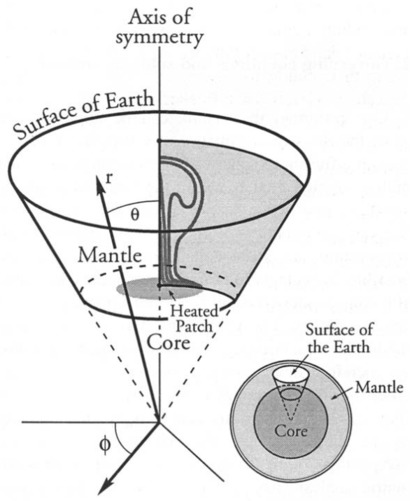
\includegraphics[width=5cm]{images/axisymmetry/keki97}\\
{\captionfont Taken from Kellogg \& King (1997) \cite{keki97}.}
\end{center}

Assuming the flow velocity does not depend on $\phi$ ($\partial_\phi =0$) and therefore also that $\upnu_\phi=0$
\[
0=-\frac{\partial p}{\partial r} + f_r + \eta \left(\Delta v_r - \frac{2v_r}{r^2} -\frac{2}{r^2} \frac{\partial v_\theta}{\partial \theta} - \frac{2 v_\theta \cot \theta }{r^2} \right)
\]
\[
0 = -\frac{1}{r} \frac{\partial p}{\partial \theta} + \eta \left(\Delta v_\theta + \frac{2}{r^2} \frac{\partial v_r}{\partial \theta}  - \frac{v_\theta}{r^2 \sin^2 \theta} \right)
\]
with
\[
\Delta = \frac{1}{r^2} \frac{\partial }{\partial r}\left( r^2 \frac{\partial }{\partial r}\right)
+\frac{1}{r^2 \sin\theta} \frac{\partial }{\partial \theta}
\left(
\sin\theta \frac{\partial }{\partial\theta}
\right)
\]



\newpage
THESE EQUATIONS SHOULD BE CHECKED and RE-CHECKED !!
\[
\Delta = \frac{1}{r^2} \frac{\partial }{\partial r}\left( r^2 \frac{\partial }{\partial r}\right)
+\frac{1}{r^2 \sin\theta} \frac{\partial }{\partial \theta}
\left(
\sin\theta \frac{\partial }{\partial\theta}
\right)
+ \frac{1}{r^2 \sin^2\theta} \frac{\partial^2 }{\partial\phi^2}
\]

THESE EQUATIONS SHOULD BE CHECKED and RE-CHECKED !!



From \cite{zebi93}:
\begin{equation}
\frac{1}{r^2} \frac{\partial}{\partial r} (r^2 \upnu_r) + 
\frac{1}{r \sin \theta} \frac{\partial}{\partial \theta} (\upnu_\theta \sin \theta)+
\frac{1}{r \sin \theta} \frac{\partial \upnu_\phi}{\partial \phi} = 0
\end{equation}
Pb with 1/r2 ??

\begin{eqnarray}
0 &=& -\frac{\partial p}{\partial r} + (1-\zeta) Ra \; r \; T + 
\frac{1}{r^2}\frac{\partial}{\partial r} \left( 2 \eta r^2 \frac{\partial \upnu_r}{\partial r} \right)
+ \frac{1}{r^2 \sin\theta} \frac{\partial}{\partial\theta} 
\left( \eta \sin\theta \frac{\partial \upnu_r}{\partial\theta} \right)
+\frac{\partial}{\partial \theta} \left(\eta \frac{\partial}{\partial r} \frac{\upnu_\theta}{r} \right)
\end{eqnarray}
where $\zeta=R_i/R_o$


The dimensional form of the energy equation in a spherical axisymmetric geometry is given by
(assuming the conductivity $k$ to be constant):
\[
\rho C_p \left( \frac{\partial T}{\partial t}  + 
\upnu_r \frac{\partial T}{\partial r} + \frac{\upnu_\theta}{r} \frac{\partial T}{\partial \theta}
\right)
=
k \frac{1}{r^2} \frac{\partial}{\partial r} \left( r^2 \frac{\partial T}{\partial r} \right)
+
k \frac{1}{r^2 \sin\theta} 
\frac{\partial}{\partial \theta} \left( \sin\theta \frac{\partial T}{\partial \theta}  \right) 
...
\]

THESE EQUATIONS SHOULD BE CHECKED and RE-CHECKED !!





\newpage
%---------------------------------
\subsection{The Boussinesq approximation}
\index{general}{Boussinesq Approximation}

As nicely explained in Spiegel \& Veronis \cite{spve60}: "In the study of problems of thermal convection it is a frequent practice to simplify the basic equations by introducing certain approximations which are attributed to
Boussinesq (1903). The Boussinesq approximations can best be summarized by two
statements: 
\begin{enumerate}
\item The fluctuations in density which appear with the advent of motion
result principally from thermal (as opposed to pressure) effects. 
\item In the equations
for the rate of change of momentum and mass, density variations may be neglected except
when they are coupled to the gravitational acceleration in the buoyancy force."
\end{enumerate}
Note that their paper examines the Boussinesq approximation for compressible fluids.  

[from \aspect{} manual]
The Boussinesq approximation assumes that the density can be
considered constant in all occurrences in the equations with the exception of
the buoyancy term on the right hand side of \eqref{eq:stokes-1}. The primary
result of this assumption is that the continuity equation \eqref{eq:stokes-2}
will now read
\[
{\bm \nabla}\cdot{\bm v} = 0
\]
This implies that the strain rate tensor is deviatoric.
Under the Boussinesq approximation, the equations are much simplified:

\begin{align}
  \label{eq:stokes-1}
  -\nabla \cdot \left[2\eta \dot{\bm \varepsilon}(\bm v)
                \right] + \nabla p &=
  \rho \bm g
  &
  & \textrm{in $\Omega$},
  \\
  \label{eq:stokes-2}
  \nabla \cdot (\rho \bm v) &= 0
  &
  & \textrm{in $\Omega$},
  \\
  \label{eq:temperature}
  \rho_0 C_p \left(\frac{\partial T}{\partial t} + \bm v\cdot\nabla T\right)
  - \nabla\cdot k\nabla T
  &=
  \rho H
  &
  & \textrm{in $\Omega$}
\end{align}
Note that all terms on the rhs of the temperature equations have disappeared, with the exception 
of the source term.


%---------------------------------
\subsection{The Extended Boussinesq approximation}
\index{general}{Extended Boussinesq Approximation}
\index{general}{EBA}


Yuen et al (2007) \cite{yumc07} state that "the background of the extended Boussinesq 
equations can be found described in 
Christensen and Yuen (1985) \cite{chyu85} and more completely in Matyska and Yuen (2007) \cite{mayu07}.

\Literature \cite{hayk91,hayk93}




\newpage
%%%%%%%%%%%%%%%%%%%%%%%%%%%%%%%%%%%%%%%%%%%%%%%%%%%%%%%%%%%%%%%%%%%%%%%%%%%%%%%%%%%%%%%%%%55
\subsection{Stokes equation for elastic medium}

What follows is mostly borrowed from Becker \& Kaus lecture notes.

%\begin{tabular}{|l|l|l|}
%\hline
%${\bm u}       $ & displacement vector &   \\
%${\bm \sigma}  $ & full stress tensor  & Pa\\
%${\bm \epsilon}$ & strain tensor       &   \\
%${\bm 1}       $ & unit tensor         &   \\
%${\bm f}       $ & body forces         &   \\
%\hline
%\end{tabular}

The strong form of the PDE that governs force balance in a medium is given by
\[
\vec{\nabla}\cdot{\bm \sigma}  + \vec{f} = \vec{0}
\]
where ${\bm \sigma}$ is the stress tensor and $\vec{f}$ is a body force.

The stress tensor is related to the strain tensor through the generalised 
Hooke's law\footnote{\url{https://en.wikipedia.org/wiki/Hooke's_law}}:
\begin{equation}
\sigma_{ij}=\sum_{kl}C_{ijkl}\varepsilon_{kl} 
\qquad
\text{or}
\qquad
{\bm \sigma} = {\bm C} : {\bm \varepsilon}
\label{eq:oone}
\end{equation}
where ${\bm C}$ is the fourth-order elastic tensor.

Due to the inherent symmetries of ${\bm \sigma}$, ${\bm \varepsilon}$, and ${\bm C}$, 
only 21 elastic coefficients of the latter are independent. 
For isotropic media (which have the same physical properties in any direction), ${\bm C}$ 
can be reduced to only two independent numbers (for example the bulk modulus $K$ and the shear modulus $G$ 
that quantify the material's resistance to changes in volume and to shearing deformations, respectively). 

One often then write Eq.~\eqref{eq:oone} as follows:
%\sigma_{ij}=\lambda \varepsilon_{kk} \delta_{ij} + 2\mu \varepsilon_{ij}

\begin{mdframed}[backgroundcolor=blue!5]
\begin{equation}
{\bm \sigma} = \lambda (\vec{\nabla}\cdot\vec{u}) {\bm 1} + 2\mu {\bm \varepsilon}   \label{eq:twoELAST}
\end{equation}
\end{mdframed}
where $\lambda$ is the Lam\'e parameter and $\mu$ is the shear modulus\footnote{It is also sometimes written $G$}.
The term $\vec{\nabla}\cdot\vec{u}$ is the isotropic dilation.

\index{general}{Lam\'e Parameter} 
\index{general}{Shear Modulus}

The strain tensor is related to the displacement as follows: \index{general}{Strain Tensor}
\[
{\bm \varepsilon} = \frac{1}{2}(\vec{\nabla}\vec{u} + (\vec{\nabla}\vec{u})^T)
\]
The incompressibility (or bulk modulus) $K$ is defined as $p=-K \vec{\nabla}\cdot\vec{u}$ 
where $p$ is the pressure with \index{general}{Bulk Modulus}
\begin{eqnarray}
p&=&-\frac{1}{3} \text{tr}({\bm \sigma}) \nonumber\\
 &=& -\frac{1}{3} [ \lambda (\vec{\nabla}\cdot\vec{u}) \text{tr}[{\bm 1}] + 2 \mu \text{tr}[{\bm \varepsilon}]] \nonumber\\
 &=& -\frac{1}{3} [ \lambda (\vec{\nabla}\cdot\vec{u})  3  + 2 \mu  (\vec{\nabla}\cdot\vec{u}) ] \nonumber\\
 &=& -\left[ \lambda + \frac{2}{3} \mu \right] (\vec{\nabla}\cdot\vec{u})  
\end{eqnarray}
so that 
\begin{mdframed}[backgroundcolor=blue!5]
\[
p=-K \vec{\nabla}\cdot\vec{u} 
\qquad
\text{with}
\qquad
K=\lambda+\frac{2}{3}\mu
\]
\end{mdframed}


%or
%\[
%\mu=\frac{3K(1-2\nu)}{2(1+\nu)}
%\]


\begin{remark}
Eq. (\ref{eq:oone}) and (\ref{eq:twoELAST}) are analogous to the ones that one has to solve
in the context of viscous flow using the penalty method. In this case $\lambda$ is the penalty coefficient, 
${\bm u}$ is the velocity, and $\mu$ is then the dynamic viscosity.
\end{remark}

The Lam\'e parameter and the shear modulus are also linked to $\nu$ the poisson ratio, 
and $E$, Young's modulus: \index{general}{Poisson Ratio} \index{general}{Young's Modulus}
\[
\lambda=\mu\frac{2\nu}{1-2\nu}
=\frac{\nu E}{(1+\nu)(1-2\nu)}
\quad\quad
{\rm with}
\quad\quad
E=2\mu(1+\nu)
\]
The shear modulus, expressed often in GPa, describes the material's response to shear stress.
The poisson ratio describes the response in the direction orthogonal to uniaxial stress.
The Young modulus, expressed in GPa, describes the material's strain response to uniaxial stress in the 
direction of this stress.


%%%%%%%%%%%%%%%%%%%%%%%%%%%%%%%%%%%%%%%%%%%%%%%%%%%%%%%%%%%%%%%%%%55
\newpage
\subsection{The strain rate tensor in all coordinate systems}

The strain rate tensor $\dot{\bm\varepsilon}$ is given by
\begin{equation}
\dot{\bm \varepsilon}({\vec \upnu}) = \frac{1}{2}( {\vec \nabla}{\vec \upnu}+ ({\vec \nabla}{\vec \upnu})^T) 
\end{equation}

%.....................................
\subsubsection{Cartesian coordinates}
\begin{eqnarray}
\dot\varepsilon_{xx} &=& \frac{\partial u}{\partial x} \\
\dot\varepsilon_{yy} &=& \frac{\partial v}{\partial y} \\
\dot\varepsilon_{zz} &=& \frac{\partial w}{\partial z} \\
\dot\varepsilon_{yx} =
\dot\varepsilon_{xy} &=& \frac{1}{2} \left( \frac{\partial u}{\partial y} + \frac{\partial v}{\partial x}  \right)\\
\dot\varepsilon_{zx} =
\dot\varepsilon_{xz} &=& \frac{1}{2} \left( \frac{\partial u}{\partial z} + \frac{\partial w}{\partial x}  \right)\\
\dot\varepsilon_{zy} =
\dot\varepsilon_{yz} &=& \frac{1}{2} \left( \frac{\partial v}{\partial z} + \frac{\partial w}{\partial y}  \right)
\end{eqnarray}

%.....................................
\subsubsection{Polar coordinates}

\begin{eqnarray}
\dot\varepsilon_{rr} 
&=& \frac{\partial \upnu_r}{\partial r} \\
\dot\varepsilon_{\theta\theta} 
&=& \frac{\upnu_r}{r} + \frac{1}{r} \frac{\partial \upnu_\theta}{\partial \theta}  \\
\dot\varepsilon_{\theta r} = \dot\varepsilon_{r\theta} 
&=& \frac{1}{2} \left(   \frac{\partial \upnu_\theta}{\partial r} - \frac{\upnu_\theta}{r} 
+\frac{1}{r} \frac{\partial \upnu_r}{\partial \theta}  \right) 
\end{eqnarray}

%.....................................
\subsubsection{Cylindrical coordinates}

\begin{eqnarray}
\dot\varepsilon_{rr} 
&=& \frac{\partial \upnu_r}{\partial r} 
\\
\dot\varepsilon_{\theta\theta} 
&=& \frac{\upnu_r}{r} + \frac{1}{r} \frac{\partial \upnu_\theta}{\partial \theta}  
\\
\dot\varepsilon_{\theta r} = \dot\varepsilon_{r\theta} 
&=& \frac{1}{2} \left(   \frac{\partial \upnu_\theta}{\partial r} - \frac{\upnu_\theta}{r} 
+\frac{1}{r} \frac{\partial \upnu_r}{\partial \theta}  \right)
\\
\dot\varepsilon_{zz} 
&=& \frac{\partial \upnu_z}{\partial z} 
\\
\dot{\varepsilon}_{rz} = \dot{\varepsilon}_{zr} 
&=& \frac{1}{2}\left( \frac{\partial \upnu_r}{\partial z} + \frac{\partial \upnu_z}{\partial r}  \right) 
\\
\dot{\varepsilon}_{\theta z} = \dot{\varepsilon}_{z \theta} &=& \frac{1}{2}\left( 
\frac{1}{r} \frac{\partial \upnu_z}{\partial \theta} + \frac{\partial \upnu_\theta}{\partial z}  \right) 
\end{eqnarray}

%.....................................
\subsubsection{Spherical coordinates}

\begin{eqnarray}
\dot\varepsilon_{rr} 
&=& \frac{\partial \upnu_r}{\partial r} \\
\dot\varepsilon_{\theta\theta} 
&=& \frac{\upnu_r}{r} + \frac{1}{r} \frac{\partial \upnu_\theta}{\partial \theta}  \\
\dot\varepsilon_{\phi\phi} 
&=& \frac{1}{r \sin\theta} \frac{\partial \upnu_\phi}{\partial \phi} +
\frac{\upnu_r}{r} +\frac{\upnu_\theta \cot \theta}{r} \\
\dot\varepsilon_{\theta r} = \dot\varepsilon_{r\theta}   
&=& \frac{1}{2} \left( r \frac{\partial}{\partial r} (\frac{\upnu_\theta}{r} ) 
+\frac{1}{r} \frac{\partial \upnu_r}{\partial \theta} \right) \\
\dot\varepsilon_{\phi r} = \dot\varepsilon_{r\phi}      
&=&  \frac{1}{2} \left(  \frac{1}{r \sin\theta} \frac{\partial \upnu_r}{\partial \phi} 
+ r \frac{\partial }{\partial r} (\frac{\upnu_\phi}{r}) \right)  \\
\dot\varepsilon_{\phi \theta} = \dot\varepsilon_{\theta\phi} 
&=& \frac{1}{2} \left( \frac{\sin \theta}{r} \frac{\partial }{\partial \theta} (\frac{\upnu_\phi}{\sin\theta}) + \frac{1}{r \sin\theta} \frac{\partial \upnu_\theta}{\partial \phi}    \right) 
\end{eqnarray}



\newpage
%-------------------------------
\subsection{Boundary conditions}

%wiki
In mathematics, the Dirichlet (or first-type) 
boundary condition is a type of boundary condition, named after Peter Gustav Lejeune Dirichlet.
When imposed on an ODE or PDE, it specifies the values that a solution needs 
to take along the boundary of the domain.
Note that a Dirichlet boundary condition may also be referred to as a fixed boundary condition. 

The Neumann (or second-type) boundary condition is a type of boundary condition, 
named after Carl Neumann. When imposed on an ordinary or a partial differential equation, 
the condition specifies the values in which the derivative of a solution is 
applied within the boundary of the domain.

It is possible to describe the problem using other boundary conditions: 
a Dirichlet boundary condition specifies the values of the solution itself 
(as opposed to its derivative) on the boundary, whereas the Cauchy boundary condition, mixed boundary condition and Robin boundary condition are all different types of combinations of the Neumann and Dirichlet boundary conditions.

\index{general}{Dirichlet Boundary Condition}
\index{general}{Neumann Boundary Condition}

%....................................
\subsubsection{The Stokes equations}

You may find the following terms in the computational geodynamics literature:

\begin{itemize}
\item { free surface}: this means that no force is acting on the surface, i.e. ${\bm \sigma}\cdot {\vec n}={\vec 0}$. It is usually used on the top boundary of the domain and allows for topography evolution.
\item { free slip}: ${\vec \upnu}\cdot \vec n = 0$ and $({\bm \sigma}\cdot{\vec n})\times {\vec n}={\vec 0}$. This condition ensures a frictionless flow parallel to the boundary where it is prescribed.
\item { no slip}: this means that the velocity (or displacement) is exactly zero on the boundary, i.e. ${\vec \upnu}={\vec 0}$.
\item { prescribed velocity}: ${\vec \upnu}={\vec \upnu}_{bc}$
\item stress b.c.: 
\item open .b.c.: see fieldstone 29. 
\end{itemize}

%....................................
\subsubsection{The heat transport equation}

There are two types of boundary conditions for this equation: temperature boundary conditions (Dirichlet boundary conditions) and heat flux boundary conditions (Neumann boundary conditions). 

\newpage
%------------------------------------------
\subsection{Meaningful physical quantities}

\begin{itemize}
\item \underline{Velocity} $\vec \upnu (\text{m/s})$: This is a vector quantity and both magnitude and direction are needed to define it. It is the rate of change of position with respect to a frame of reference.
\item \underline{Root mean square velocity} $\upnu_{rms} (\text{m/s})$: 
\begin{equation}
\upnu_{rms} = \left ( \frac{\int_\Omega |{\vec \upnu}|^2 \;  d \Omega}{\int_\Omega d\Omega }  \right )^{1/2}
=\left ( \frac{1}{V_\Omega} \int_\Omega |{\vec \upnu}|^2 \;  d \Omega \right )^{1/2} \label{eqVrms}
\end{equation}
\begin{remark}
$V_\Omega$ is usually computed numerically at the same time $\upnu_{vrms}$ is computed.
\end{remark}
In Cartesian coordinates, for a cuboid domain of size $Lx\times L_y \times Lz$, 
the $\upnu_{rms}$ is simply given by:
\begin{equation}
\upnu_{rms}  = \left ( \frac{1}{L_xL_yL_z} \int_0^{L_x}\int_0^{L_y}\int_0^{L_z} 
(u^2 + v^2 + w^2) dxdydz  \right )^{1/2}
\end{equation}
In the case of an annulus domain, although calculations are carried out 
in Cartesian coordinates, it makes sense
to look at the radial velocity component $\upnu_r$ and the tangential velocity 
component $\upnu_\theta$, and their respective
root mean square averages:
\begin{equation}
\upnu_r|_{rms}  =\left ( \frac{1}{V_\Omega} \int_\Omega v_r^2 \;  d \Omega \right )^{1/2} \label{eqVrVrms}
\end{equation}
\begin{equation}
\upnu_\theta|_{rms}  = \left ( \frac{1}{V_\Omega} \int_\Omega v_\theta^2 \;  d \Omega \right )^{1/2} \label{eqThetaVrms}
\end{equation}


\item \underline{Pressure} $p (\text{Pa})$:
\item \underline{Stress tensor} ${\bm \sigma}$ (Pa): \index{general}{Stress Tensor}
\item \underline{Strain tensor} ${\bm \varepsilon}$ (dimensionless): \index{general}{Strain Tensor}
\item \underline{Strain rate tensor} $ \dot{\bm \varepsilon} (\text{s}^{-1}$): \index{general}{Strain Rate Tensor}
\item \underline{Rayleigh number} $Ra$ (X): \index{general}{Rayleigh Number}
It is a dimensionless number that expresses the	ratio of the driving forces to the opposing forces.
The buoyancy force comes from the volumetric thermal expansion while the viscous forces and 
the heat diffusivity oppose convection (the latter one smoothes out thermal gradients). 

The Rayleigh number for convection driven by a constant temperature hot base and a cold surface
in a domain of thickness $D$ is:
\[
Ra 
= \frac{\rho_0 g \alpha D^3 }{\eta \kappa}  \cdot  \Delta T
= \frac{\rho_0^2 C_p g \alpha D^3 \Delta T}{\eta k}
\]
The Rayleigh number for convection driven by a hot base (constant basal heat flow $q_b$)
and a colder surface is:
\[
Ra = \frac{\rho_0 g \alpha D^3}{\eta \kappa } \cdot  \frac{q_b D}{k}
\]  
The Rayleigh number for convection driven by internal heating $H$ (production per cubic meter) is:
\[
Ra = \frac{\rho_0 g \alpha D^3}{\eta \kappa} \cdot  \frac{H D^2}{k }
\]
The Rayleigh number for convection driven by both basal heat flow and internal heating is:	
\[
Ra = \frac{\rho_0 g \alpha D^3}{\eta \kappa} \cdot  \frac{q_b D + H D^2}{k }
\]
For convection to occur, the Rayleigh number must be larger than the so-called critical 
Rayleigh number, which ranges from 600 to 3000 (it depends on the boundary conditions and the 
geometry).
\index{general}{Critical Rayleigh Number}


\item \underline{Prandtl number} $Pr$ (X): \index{general}{Prandtl Number} It is named after the German physicist 
Ludwig Prandtl and is defined as the ratio of momentum diffusivity to thermal diffusivity. It is given as: 
\[
Pr = \frac{\text{momentum diffusivity}}{\text{thermal diffusivity}} = \frac{\eta/\rho}{k/(\rho C_p)}= \frac{\eta C_p}{k}
\]
For Earth materials, we have $Pr \sim (10^{21} 1000)/3 >> 1$, which means that momentum diffusivity dominates.

%..........................................
\item \underline{Nusselt number} $N_u$ (X): \index{general}{Nusselt Number}  the Nusselt number (Nu) 
is the ratio of convective to conductive heat transfer across (normal to) the boundary. 
The conductive component is measured under the same conditions as the heat convection 
but with a (hypothetically) stagnant (or motionless) fluid.

In practice the Nusselt number Nu of a layer (typically the mantle of a planet) is defined as follows:
\begin{equation}
\text{Nu} = \frac{q}{q_c}
\end{equation} 
where $q$ is the heat transferred by convection while $q_c=k \Delta T /D$ 
is the amount of heat that would be conducted through a layer of
thickness $D$ with a temperature difference $\Delta T$ across it with 
$k$ being the thermal conductivity.

For 2D Cartesian systems of size ($L_x$,$L_y$) the Nu is computed \cite{blbc89}
\[
\text{Nu} = 
 \frac{\frac{1}{L_x}\int_{0}^{L_x} k \frac{\partial T}{\partial y}(x,y=L_y) dx }
{-\frac{1}{L_x}\int_0^{L_x} k T(x,y=0) /L_y dx}
=-L_y \frac{\int_{0}^{L_x} \frac{\partial T}{\partial y}(x,y=L_y) dx }{\int_0^{L_x} T(x,y=0) dx}
\]
i.e. it is the mean surface temperature gradient
over the mean bottom temperature.

\todo[inline]{finish. not happy with definition. Look at literature}

Note that in the case when no convection takes place then the measured heat flux at the top is 
the one obtained from a purely conductive profile which yields Nu=1.

Note that a relationship Ra $\propto$ Nu$^\alpha $ exists between the Rayleigh number Ra and the Nusselt number Nu in convective systems, see \cite{wodd09} and references therein. 

Turning now to cylindrical geometries with inner radius $R_1$ and outer radius $R_2$, we define $f=R_1/R_2$. A small value of $f$ corresponds to a high
degree of curvature. We assume now that $R_2-R_1=1$, so that $R_2=1/(1-f)$ and $R_1=f/(1-f)$. 
Following \cite{jarv93}, the Nusselt number at the inner and outer boundaries are:
\begin{equation}
\boxed{
\text{Nu}_{inner} = \frac{f \ln f}{1-f} \frac{1}{2\pi} \int_0^{2\pi} \left( \frac{\partial T}{\partial r} \right)_{r=R_1} d\theta
}
\label{eqNuAnnIn}
\end{equation}
\begin{equation}
\boxed{
\text{Nu}_{outer} = \frac{\ln f}{1-f} \frac{1}{2\pi} \int_0^{2\pi} \left( \frac{\partial T}{\partial r} \right)_{r=R_2} d\theta
}
\label{eqNuAnnOut}
\end{equation}

Note that a conductive geotherm in such an annulus between temperatures $T_1$ and $T_2$ is given by 
\[
T_c(r)=\frac{\ln (r/R_2)}{\ln(R_1/R_2)} = \frac{\ln(r(1-f))}{\ln f}
\]
so that 
\[
\frac{\partial T_c}{\partial r} = \frac{1}{r}\frac{1}{\ln f} 
\]
We then find:
\begin{eqnarray}
\text{Nu}_{inner} 
&=& \frac{f \ln f}{1-f} \frac{1}{2\pi} \int_0^{2\pi} \left( \frac{\partial T_c}{\partial r} \right)_{r=R_1} d\theta
= \frac{f \ln f}{1-f} \frac{1}{R_1}\frac{1}{\ln f} 
= 1 \\
\text{Nu}_{outer} 
&=& \frac{\ln f}{1-f} \frac{1}{2\pi} \int_0^{2\pi} \left( \frac{\partial T_c}{\partial r} \right)_{r=R_2} d\theta 
= \frac{\ln f}{1-f} \frac{1}{R_2}\frac{1}{\ln f} = 1 
\end{eqnarray}
As expected, the recovered Nusselt number at both boundaries is exactly 1 when the temperature field is
given by a steady state conductive geotherm.

\todo[inline]{derive formula for Earth size R1 and R2}

\Literature \cite{hohr87}
 
%..........................................
\item \underline{Temperature} (K):
\item \underline{(Dynamic) Viscosity} (Pa.s): For air it is roughly $10^{-5}$Pa.s, about $10^{-3}$Pa.s for water, about $10^{10}$Pa.s for ice and about $10^{17}$Pa.s for salt. 



\item \underline{Density} (kg/m$^3$):
\item \underline{Heat capacity} $C_p$ ($J.K^{-1}$): 
It is the measure of the heat/energy required to increase the 
temperature of a unit quantity of a substance by unit degree. Note that the specific heat capacity $c_P$ of a 
substance is the heat capacity of a sample of the substance divided by the mass of the sample, with units $J\cdot K\cdot kg^{-1}$.

\item \underline{Heat conductivity}, or thermal conductivity $k$ ($W.m^{-1}.K^{-1}$). It is the 
property of a material that indicates its ability to conduct heat. It appears primarily in 
Fourier's Law for heat conduction.
Note that it is a function of temperature, especially in mantle convection settings \cite{mika13}. 
See also \cite{boca99} and refs therein. Note also that it can be a tensorial quantity in 
anisotropic context. 

\item \underline{Heat diffusivity}: $\kappa=k/(\rho C_p)$ ($m^2.s^{-1}$). Substances with high thermal diffusivity rapidly adjust their temperature to that of their surroundings, because they 
conduct heat quickly in comparison to their volumetric heat capacity or 'thermal bulk'.
\item \underline{thermal expansion} $\alpha$ (K$^{-1}$): it is the tendency of a matter to change in volume in response to a change in temperature. Note that it is a function of temperature, especially in mantle convection settings \cite{mika13}.

\item \underline{Urey Ratio}: mantle heat production divided by heat loss) is a key constraint for thermal history models. Recent Urey ratio estimates are in the range of 0.21–0.49. \cite{lecm11}

\item \underline{Shear modulus}: modulus of rigidity, usually expressed in GPa. It describes the 
material response to shear stress.

\item \underline{Poisson ratio}: response in the direction orthogonal to uniaxial stress.

\item \underline{Young's modulus}: describes the material strain response to uniaxial stress
in the direction of this stress, usually expressed in GPa.

\item \underline{Average viscosity}: following Christensen (1983) \cite{chri83b}, one can compute the averaged
viscosity in a domain as follows:
\begin{equation}
\langle \eta \rangle = \frac{\int_V \eta \dot{\varepsilon}_e^2 dV}{\int_V  \dot{\varepsilon}_e^2 dV }
\label{eq:avrgeta}
\end{equation}


\end{itemize}


\todo[inline]{check aspect manual The 2D cylindrical shell benchmarks by Davies et al. 5.4.12}


%------------------------------------------------------
\subsection{Principal stress and principal invariants} \label{sec:princ_stress}

\index{general}{Maximum Shear Stress} 
\index{general}{Principal Stress}

As seen before (see Section~\ref{sec:stresstensor}) 
the stress tensor is a symmetric $3\times3$ real matrix, and linear algebra tells us that it 
therefore has three mutually orthogonal unit-length eigenvectors $\vec{n}_{1}$, $\vec{n}_{2}$, 
$\vec{n}_{3}$ and three real eigenvalues $\lambda _{1},\lambda _{2},\lambda _{3}$ 
such that ${\bm \sigma}\cdot \vec{n}_i=\lambda_{i} \vec{n}_{i}$.

%from wiki stress 
As a consequence, in a coordinate system with axes $\vec{n}_{1},\vec{n}_{2},\vec{n}_{3}$, 
the stress tensor is a diagonal matrix, and has only the three normal components $\lambda _{1},\lambda _{2},\lambda _{3}$
i.e. the principal stresses. If the three eigenvalues are equal, the stress is an isotropic compression or tension, always perpendicular to any surface, there is no shear stress, and the tensor is a diagonal matrix in any coordinate frame.

\subsubsection{In two dimensions}

We are looking for the stress tensor eigenvector vector $\vec{n}=(n_x,n_y)$ associated to the
eigenvalue $\lambda$ such that 
\[
\left(
\begin{array}{cc}
\sigma_{xx} & \sigma_{xy} \\
\sigma_{xy} & \sigma_{yy} 
\end{array}
\right)
\cdot
\left(
\begin{array}{c}
n_x \\ n_y
\end{array}
\right)
=
\lambda
\left(
\begin{array}{c}
n_x \\ n_y
\end{array}
\right)
\]
or,
\[
\left(
\begin{array}{cc}
\sigma_{xx} & \sigma_{xy} \\
\sigma_{xy} & \sigma_{yy} 
\end{array}
\right)
\cdot
\left(
\begin{array}{c}
n_x \\ n_y
\end{array}
\right)
-
\left(
\begin{array}{cc}
\lambda & 0 \\ 
0 & \lambda 
\end{array}
\right)
\cdot
\left(
\begin{array}{c}
n_x \\ n_y
\end{array}
\right)
= \vec{0}
\]
i.e.,
\[
\left(
\begin{array}{cc}
\sigma_{xx}-\lambda  & \sigma_{xy} \\
\sigma_{xy} & \sigma_{yy} -\lambda 
\end{array}
\right)
\cdot
\left(
\begin{array}{c}
n_x \\ n_y
\end{array}
\right)
= \vec{0}
\]

which yields
\[
(\sigma_{xx}-\lambda)(\sigma_{yy}-\lambda)-\sigma_{xy}^2 =0
\]
or, 
\[
\lambda^2 - (\sigma_{xx}+\sigma_{yy}) \lambda   + (\sigma_{xx}\sigma_{yy}-\sigma_{xy}^2) =0
\]
The discriminant $\Delta$ is 
\begin{eqnarray}
\Delta 
&=& (\sigma_{xx}+\sigma_{yy})^2-4(\sigma_{xx}\sigma_{yy}-\sigma_{xy}^2)  \nn\\
&=& (\sigma_{xx}-\sigma_{yy})^2 +4\sigma_{xy}^2  \nn
\end{eqnarray}
The roots are given by:
\begin{eqnarray}
\lambda_\pm 
&=& \frac{ (\sigma_{xx}+\sigma_{yy}) \pm \sqrt{ (\sigma_{xx}-\sigma_{yy})^2 +4\sigma_{xy}^2 } }{2} \nn\\
&=& \frac{ \sigma_{xx}+\sigma_{yy}}{2} \pm \sqrt{ \left(\frac{\sigma_{xx}-\sigma_{yy}}{2}\right)^2 +\sigma_{xy}^2 } \nn
\end{eqnarray}
The two principal stresses are then:
\begin{eqnarray}
\sigma_1 &=& \frac{ \sigma_{xx}+\sigma_{yy}}{2} + \sqrt{ \left(\frac{\sigma_{xx}-\sigma_{yy}}{2}\right)^2 +\sigma_{xy}^2 } \nn\\
\sigma_2 &=& \frac{ \sigma_{xx}+\sigma_{yy}}{2} - \sqrt{ \left(\frac{\sigma_{xx}-\sigma_{yy}}{2}\right)^2 +\sigma_{xy}^2 } \nn
\end{eqnarray}
with the convention $\sigma_1>\sigma_2$.
The maximum shear stress is defined as one-half the difference between the two principal 
stresses 
\[
\tau_{\text max}=
\frac{\sigma_1-\sigma_2}{2}
=\sqrt{ \left(\frac{\sigma_{xx}-\sigma_{yy}}{2}\right)^2 +\sigma_{xy}^2 } 
\]

The eigenvector $\vec{n}_1$ corresponding to $\sigma_1$ is obtained by solving 
\[
{\bm \sigma}\cdot \vec{n}_1 = \sigma_1 \vec{n}_1
\]
and same for the other eigenvalue/vector:
\[
{\bm \sigma}\cdot \vec{n}_2 = \sigma_2 \vec{n}_2
\]
Each is a system of two equations with two unknowns. These are not difficult to solve, 
but can prove cumbersome. Note that linear algebra tells us that $\vec{n}_1\cdot\vec{n}_2=0$, 
i.e. the eigenvectors form a basis of $\mathbb{R}^2$.

This is the reason why often people go another route. One can ask the question: what is the 
value of the angle $\theta_p$ which, if used to perform a rotation of the axis system, yields 
a stress tensor that is diagonal, with the principal stresses on the diagonal?
 
\begin{center}
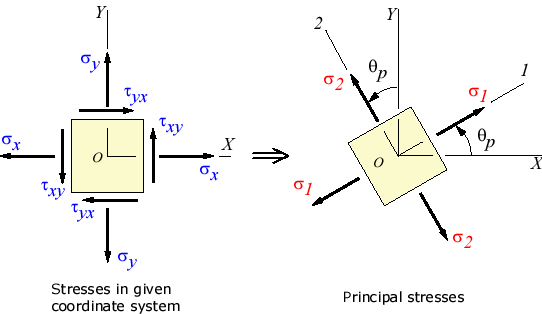
\includegraphics[width=8cm]{images/princ_stress/PrincipalStress}\\
{\scriptsize Taken from \url{https://www.efunda.com/formulae/solid_mechanics/mat_mechanics/plane_stress_principal.cfm}}
\end{center}
 
The rotation matrix is 
\[
{\bm R}=
\left(
\begin{array}{cc}
\cos\theta_p & -\sin\theta_p \\
\sin\theta_p & \cos\theta_p
\end{array}
\right)
\]
and the image of ${\bm \sigma}$ by means of the axis rotation is 
${\bm \sigma}'= {\bm R}\cdot {\bm \sigma}\cdot {\bm R}^{-1}$, i.e.
\begin{eqnarray}
{\bm \sigma}' 
&=&
\left(
\begin{array}{cc}
\cos\theta_p & -\sin\theta_p \\
\sin\theta_p & \cos\theta_p
\end{array}
\right)
\cdot
\left(
\begin{array}{cc}
\sigma_{xx} & \sigma_{xy} \\
\sigma_{xy} & \sigma_{yy} 
\end{array}
\right)
\cdot
\left(
\begin{array}{cc}
\cos\theta_p & \sin\theta_p \\
-\sin\theta_p & \cos\theta_p
\end{array}
\right) \nn\\
&=&\left(
\begin{array}{cc}
\cos\theta_p & -\sin\theta_p \\
\sin\theta_p & \cos\theta_p
\end{array}
\right)
\cdot
\left(
\begin{array}{cc}
\sigma_{xx} \cos\theta_p - \sigma_{xy} \sin\theta_p  &
\sigma_{xx} \sin\theta_p + \sigma_{xy} \cos\theta_p  \\
\sigma_{xy} \cos\theta_p - \sigma_{yy} \sin\theta_p & 
\sigma_{xy} \sin\theta_p + \sigma_{yy} \cos\theta_p 
\end{array}
\right) \nn\\
&=&
\left(
\begin{array}{cc}
\dots & 
\cos\theta_p(\sigma_{xx} \sin\theta_p + \sigma_{xy} \cos\theta_p )-
\sin\theta_p(\sigma_{xy} \sin\theta_p + \sigma_{yy} \cos\theta_p ) \\
\dots & \dots 
\end{array}
\right) \nn 
\end{eqnarray}
In the matrix above I have only computed the off diagonal term since 
we are actually looking for $\theta_p$ such that $\sigma_{xy}'=0$, or
\begin{eqnarray}
\cos\theta_p(\sigma_{xx} \sin\theta_p + \sigma_{xy} \cos\theta_p )-
\sin\theta_p(\sigma_{xy} \sin\theta_p + \sigma_{yy} \cos\theta_p ) &=& 0 \nn\\
\sin\theta_p \cos\theta_p (\sigma_{xx}-\sigma_{yy}) + ( \cos^2\theta_p -\sin^2\theta_p )\sigma_{xy} &=& 0 \nn 
\end{eqnarray}
and then 
\[
\frac{ \sin\theta_p \cos\theta_p}{ \cos^2\theta_p -\sin^2\theta_p }
= \frac{\sigma_{xy}}{ \sigma_{xx}-\sigma_{yy} }
\]
The left hand term is actually a trigonometric 
identity\footnote{\url{https://en.wikipedia.org/wiki/List_of_trigonometric_identities}}:
\[
\frac{ \sin\theta_p \cos\theta_p}{ \cos^2\theta_p -\sin^2\theta_p } = \frac{1}{2} \tan 2\theta_p
\]
and finally:
\[
\tan 2\theta_p = \frac{ 2\sigma_{xy}}{ \sigma_{xx}-\sigma_{yy} }
\qquad
\text{or}
\qquad
\theta_p = \frac{1}{2} \tan^{-1} \frac{ 2\sigma_{xy}}{ \sigma_{xx}-\sigma_{yy} }
\]
Once $\theta_p$ has been found the other direction is given by $\theta_p +\pi/2$.

\vspace{.5cm}

\noindent \underline{Example}: Let us assume a diagonal stress tensor of the form 
\[
{\bm \sigma} = 
\left(
\begin{array}{cc}
a & 0 \\
0 & b
\end{array}
\right)
\]
then $\tan 2\theta_p = 0$, and then $\theta_p=0$. The principal directions are the horizontal and 
vertical directions, i.e. the Cartesian axis system, which is consistent.

%...................................... 
\subsubsection{In three dimensions}

We are looking for the stress tensor eigenvector vector $\vec{n}=(n_x,n_y,n_z)$ associated to the
eigenvalue $\lambda$ such that 
\[
\left(
\begin{array}{ccc}
\sigma_{xx} & \sigma_{xy} & \sigma_{xz} \\
\sigma_{xy} & \sigma_{yy} & \sigma_{yz} \\
\sigma_{xz} & \sigma_{yz} & \sigma_{zz}
\end{array}
\right)
\cdot
\left(
\begin{array}{c}
n_x \\ n_y \\ n_z
\end{array}
\right)
=
\lambda
\left(
\begin{array}{c}
n_x \\ n_y \\ n_z
\end{array}
\right)
\]
or,
\[
\left(
\begin{array}{ccc}
\sigma_{xx} & \sigma_{xy} & \sigma_{xz} \\
\sigma_{xy} & \sigma_{yy} & \sigma_{yz} \\
\sigma_{xz} & \sigma_{yz} & \sigma_{zz}
\end{array}
\right)
\cdot
\left(
\begin{array}{c}
n_x \\ n_y \\ n_z
\end{array}
\right)
-
\left(
\begin{array}{ccc}
\lambda & 0 & 0\\ 
0 & \lambda  & 0 \\
0 & 0 & \lambda 
\end{array}
\right)
\cdot
\left(
\begin{array}{c}
n_x \\ n_y \\ n_z
\end{array}
\right)
= \vec{0}
\]

\[
\left(
\begin{array}{ccc}
\sigma_{xx}-\lambda & \sigma_{xy} & \sigma_{xz} \\
\sigma_{xy} & \sigma_{yy}-\lambda & \sigma_{yz} \\
\sigma_{xz} & \sigma_{yz} & \sigma_{zz} -\lambda
\end{array}
\right)
\cdot
\left(
\begin{array}{c}
n_x \\ n_y \\ n_z
\end{array}
\right)
= \vec{0}
\]
Non-trivial solutions of this equation require 
\[
\left|  
\begin{array}{ccc}
\sigma_{xx}-\lambda & \sigma_{xy} & \sigma_{xz} \\
\sigma_{xy} & \sigma_{yy}-\lambda & \sigma_{yz} \\
\sigma_{xz} & \sigma_{yz} & \sigma_{zz} -\lambda
\end{array}
\right|
=0
\]
Expanding the determinant results in the following cubic equation:
\begin{eqnarray}
0 
&=&
(\sigma_{xx}-\lambda) [ ( \sigma_{yy}-\lambda )( \sigma_{zz} -\lambda)- \sigma_{yz}^2]
- \sigma_{xy} [ \sigma_{xy} ( \sigma_{zz} -\lambda) - \sigma_{yz} \sigma_{xz} ] 
+ \sigma_{xz} [ \sigma_{xy}  \sigma_{yz} - (\sigma_{yy}-\lambda )  \sigma_{xz} ]  \nn\\
&=& (\sigma_{xx}-\lambda) [ \sigma_{yy}\sigma_{zz} -\lambda (\sigma_{yy}+ \sigma_{zz})+ \lambda ^2- \sigma_{yz}^2]
- \sigma_{xy} [ \sigma_{xy} ( \sigma_{zz} -\lambda) - \sigma_{yz} \sigma_{xz} ] 
+ \sigma_{xz} [ \sigma_{xy}  \sigma_{yz} - (\sigma_{yy}-\lambda )  \sigma_{xz} ] \nn\\
&=& -\lambda^3
+ (\sigma_{xx} + \sigma_{yy} + \sigma_{zz} )\lambda^2
+ (-\sigma_{yy}\sigma_{zz} -\sigma_{xx}\sigma_{yy} -\sigma_{xx}\sigma_{zz} 
  +\sigma_{yz}^2 +\sigma_{xy}^2 + \sigma_{xz}^2 )\lambda
+ det({\bm \sigma}) \nn
\end{eqnarray}
or, after multiplying the last line by -1,
\begin{equation}
\lambda^3 - K_1({\bm \sigma}) \lambda^2 + K_2({\bm \sigma}) \lambda -K_3({\bm \sigma})=0
\end{equation}
with:
\begin{eqnarray}
K_1({\bm \sigma}) &=& \sigma_{xx}+\sigma_{yy}+\sigma_{zz}\nn\\
K_2({\bm \sigma}) &=& \sigma_{xx}\sigma_{yy}+\sigma_{yy}\sigma_{zz}+\sigma_{xx}\sigma_{zz}
-\sigma_{xy}^2 -\sigma_{xz}^2 -\sigma_{yz}^2 \nn\\
K_3({\bm \sigma}) 
&=& \det ({\bm \sigma}) \nn\\
&=& \sigma_{xx}\sigma_{yy}\sigma_{zz}-\sigma_{xx}\sigma_{yz}^2
-\sigma_{xy}^2\sigma_{zz}+\sigma_{xy}\sigma_{yz}\sigma_{xz}
+\sigma_{xz}\sigma_{xy}\sigma_{yz}-\sigma_{xz}^2\sigma_{yy} \nn\\
&=& \sigma_{xx}\sigma_{yy}\sigma_{zz}
+2\sigma_{xy}\sigma_{yz}\sigma_{xz}
-( \sigma_{xx}\sigma_{yz}^2 +  \sigma_{zz} \sigma_{xy}^2 + \sigma_{yy}\sigma_{xz}^2 )
\end{eqnarray}
\index{general}{Principal Invariants}
$K_1$, $K_2$ and $K_3$ are called {\bf principal}
invariants\footnote{\url{https://en.wikipedia.org/wiki/Invariants_of_tensors}} 
(see also Appendix A.1 of Zienkiewicz \& Taylor \cite{zita2}). 
These invariants can be written in a coordinate-free manner:
\begin{eqnarray}
K_1({\bm \sigma}) &=& tr({\bm \sigma})  \nn\\
K_2({\bm \sigma}) &=& \frac{1}{2}(  tr({\bm \sigma}) ^2 - tr({\bm \sigma}^2)  ) \nn\\
K_3({\bm \sigma}) &=& \det ({\bm \sigma}) \nn
\end{eqnarray}
and if the stress tensor is diagonal, we have
\begin{eqnarray}
K_1({\bm \sigma}) &=& \sigma_{1}+\sigma_{2}+\sigma_{3}\nn\\
K_2({\bm \sigma}) &=& \sigma_{1}\sigma_{2}+\sigma_{2}\sigma_{3}+\sigma_{1}\sigma_{3} \nn\\
K_3({\bm \sigma}) &=& \sigma_1\sigma_2\sigma_3 \nn
\end{eqnarray}
The principal invariants $K_{\{1,2,3\}}$ are related to the {\bf moment} invariants ${\cal I}_{\{1,2,3\}}$ 
(see Section~\ref{sec:invariants}) as follows (Appendix A.2 of Zienkiewicz \& Taylor \cite{zita2}):
\begin{eqnarray}
{\cal I}_1({\bm \sigma})&=& K_1({\bm \sigma}) \\ 
{\cal I}_2({\bm \sigma})&=& \frac{1}{2}K_1({\bm \sigma})^2 -K_2({\bm \sigma}) \label{eq:IK2}\\
{\cal I}_3({\bm \sigma})&=& \frac{1}{6}K_1({\bm \sigma})^3 -K_1({\bm \sigma}) K_2({\bm \sigma}) +K_3({\bm \sigma}) \label{eq:IK3}
\end{eqnarray}
Very often we will find ourselves interested in the principal components 
of the deviatoric stress tensor $\bm \tau$ so that we now have the following determinant to compute:
\[
\left|  
\begin{array}{ccc}
\tau_{xx}-\lambda & \tau_{xy} & \tau_{xz} \\
\tau_{xy} & \tau_{yy}-\lambda & \tau_{yz} \\
\tau_{xz} & \tau_{yz} & \tau_{zz} -\lambda
\end{array}
\right|
=0
\]
and therefore obtain the following cubic equation
\begin{equation}
\lambda^3 - K_1({\bm \tau}) \lambda^2 + K_2({\bm \tau}) \lambda -K_3({\bm \tau})=0
\end{equation}
By definition of a deviatoric tensor we have $K_1({\bm \tau})=0$ and then Eqs.~(\ref{eq:IK2}) and (\ref{eq:IK3}) become
\begin{eqnarray}
{\cal I}_2({\bm \tau}) &=&  - K_2({\bm \tau}) \\
{\cal I}_3({\bm \tau}) &=&  K_3({\bm \tau}) 
\end{eqnarray}
so that the cubic equation becomes
\begin{equation} 
\lambda^3 -  {\cal I}_2({\bm \tau}) \lambda -  {\cal I}_3({\bm \tau}) =0 \label{opopop}
\end{equation}
Noting the trigonometric identity\footnote{see section 7.4 of Owen \& Hinton \cite{owhi}}
\begin{equation}
\sin 3\theta = 3 \sin \theta - 4 \sin^3 \theta
\qquad
{\rm or,}
\qquad
\sin^3 \theta - \frac{3}{4}\sin \theta + \frac{1}{4} \sin 3\theta = 0\label{pc_eq2}
\end{equation}
and substituting $\lambda=r\sin \theta$ into (\ref{opopop}) we have\footnote{Note that $r$ and $\theta$ have nothing 
to do with polar, cylindrical or spherical coordinates.}
\begin{equation}
\sin^3 \theta -\frac{ {\cal I}_2({\bm \tau})   }{r^2} \sin \theta -\frac{ {\cal I}_3({\bm \tau})  }{r^3}=0\label{pc_eq3}
\end{equation}
Comparing (\ref{pc_eq2}) and (\ref{pc_eq3}) gives
\begin{eqnarray}
r&=&\frac{2}{\sqrt{3}}\sqrt{ {\cal I}_2({\bm \tau})  }\label{pc_eq4bis} \\
\sin 3 \theta &=& -\frac{4 {\cal I}_3({\bm \tau})  }{r^3}=-\frac{3\sqrt{3}}{2}\frac{ {\cal I}_3({\bm \tau}) }{ {\cal I}_2({\bm \tau}) ^{3/2}} \label{pc_eq4}
\end{eqnarray}

The so-called Lode angle  \cite{zico74} is then given by \index{general}{Lode Angle}
\begin{mdframed}[backgroundcolor=blue!5]
\begin{equation}
\theta=\frac{1}{3} \sin^{-1} \left( -\frac{3\sqrt{3}}{2} \frac{{\cal I}_3({\bm \tau})}{{\cal I}_2({\bm \tau})^{3/2}} \right)
\label{eq:lodang}
\end{equation}
\end{mdframed}
with $-\pi/6 <\theta <\pi/6 $. The very same equation is also found in Willett (1992) \cite{will92} for instance.

The first root of (\ref{pc_eq4}) with $\theta$ determined for $3\theta$ in the 
range $\pm \pi/2$ is a convenient alternative to the third invariant, ${\cal I}_3({\bm \tau})$. 
By noting the cyclic nature of $\sin (3\theta+2n \pi)$ we have immediatly the three 
(and only three) possible values of $\sin \theta $ which define the three principal stresses. 
The deviatoric principal stresses are given by $\lambda=r \sin \theta$ on substitution 
of the three values of $\sin \theta$ in turn. 

We then obtain 
\begin{equation}
\left\{
\begin{array}{c}
\tau_1 \\ \\
\tau_2 \\ \\
\tau_3
\end{array}
\right\}
= \frac{2  }{\sqrt{3}}\sqrt{ {\cal I}_2({\bm \tau})  }
\left\{
\begin{array}{c}
\sin (\theta + 2\pi/3)  \\ \\
\sin \theta   \\ \\
\sin (\theta + 4\pi/3  )
\end{array}
\right\}
\end{equation}
with $\tau_1>\tau_2>\tau_3$ and $-\pi/6 \leq \theta \leq \pi/6$. It is indeed easy to verify that 
for $-\pi/6 \leq \theta \leq \pi/6$ we have  
$\sin (\theta + 2\pi/3) > \sin \theta > \sin (\theta + 4\pi/3)$.

Finally, we wish to compute the principal stresses of the full stress tensor ${\bm \sigma}$.
In the right coordinate system both stress and deviatoric stress tensors are diagonal and 
${\bm \sigma}=-p {\bm 1} + {\bm \tau}$ writes:
\[
\left(
\begin{array}{ccc}
\sigma_1 &0 &0 \\
0& \sigma_2 &0 \\
0&0 & \sigma_3  
\end{array}
\right)
=
\left(
\begin{array}{ccc}
-p&0&0\\
0&-p&0\\
0&0&-p
\end{array}
\right)
+
\left(
\begin{array}{ccc}
\tau_1 & 0&0 \\
0& \tau_2 & 0\\
0&0 & \tau_3  
\end{array}
\right)
\]
so that (since $p=-\frac{1}{3}tr({\bm \sigma})=-\frac{1}{3}{\cal I}_1({\bm \sigma})$) 
\begin{eqnarray}
\sigma_1 &=& \tau_1 - p = \tau_1 + \frac{1}{3}{\cal I}_1({\bm \sigma})\\ 
\sigma_2 &=& \tau_2 - p = \tau_2 + \frac{1}{3}{\cal I}_1({\bm \sigma})\\ 
\sigma_3 &=& \tau_3 - p = \tau_3 + \frac{1}{3}{\cal I}_1({\bm \sigma}) 
\end{eqnarray}
and finally the total principal stresses are
\begin{equation}
\left\{
\begin{array}{c}
\sigma_1 \\ \\
\sigma_2 \\ \\
\sigma_3
\end{array}
\right\}
= \frac{2  }{\sqrt{3}}\sqrt{ {\cal I}_2({\bm \tau})  }
\left\{
\begin{array}{c}
\sin (\theta + 2\pi/3)  \\ \\
\sin \theta   \\ \\
\sin (\theta + 4\pi/3  )
\end{array}
\right\}
+
\frac{{\cal I}_1({\bm \sigma})}{3}
\left\{
\begin{array}{c}
1 \\ \\
1 \\ \\
1
\end{array}
\right\}
\end{equation}
with $\sigma_1>\sigma_2>\sigma_3$ and $-\pi/6 \leq \theta \leq \pi/6$. 
We have
\begin{eqnarray}
\sin (\theta + 2\pi/3)  
&=& \sin \theta \cos 2\pi/3 + \cos \theta \sin 2\pi/3 \nn\\
&=& -\frac{1}{2}\sin \theta  + \cos \theta \frac{\sqrt{3}}{2} \\
\sin (\theta + 4\pi/3)  
&=& \sin \theta \cos 4\pi/3 + \cos \theta \sin 4\pi/3  \nn\\
&=& -\frac{1}{2} \sin \theta - \cos \theta \frac{\sqrt{3}}{2} 
\end{eqnarray}
so that 
\begin{eqnarray}
\left\{
\begin{array}{c}
\sigma_1 \\ \\
\sigma_2 \\ \\
\sigma_3
\end{array}
\right\}
&=& \frac{2  }{\sqrt{3}}\sqrt{ {\cal I}_2({\bm \tau}) }
\left\{
\begin{array}{c}
-\frac{1}{2}\sin \theta  + \cos \theta \frac{\sqrt{3}}{2} \\ \\
\sin \theta   \\ \\
-\frac{1}{2} \sin \theta - \cos \theta \frac{\sqrt{3}}{2} 
\end{array}
\right\}
+
\frac{{\cal I}_1({\bm \sigma})}{3}
\left\{
\begin{array}{c}
1 \\ \\
1 \\ \\
1
\end{array}
\right\} \\
&=& \sqrt{ {\cal I}_2({\bm \tau}) }
\left\{
\begin{array}{c}
-\frac{1}{\sqrt{3}}\sin \theta  + \cos \theta \\ \\
\frac{2}{\sqrt{3}} \sin \theta \\ \\
-\frac{1}{\sqrt{3}}\sin \theta  - \cos \theta 
\end{array}
\right\}
+
\frac{{\cal I}_1({\bm \sigma})}{3}
\left\{
\begin{array}{c}
1 \\ \\
1 \\ \\
1
\end{array}
\right\}
\label{eq:sig123}
\end{eqnarray}





\begin{remark} The Lode angle is one of the Lode 
coordinates\footnote{\url{https://en.wikipedia.org/wiki/Lode_coordinates}},
or Haigh-Westergaard coordinates. 
\index{general}{Haigh-Westergaard Coordinates}
\index{general}{Lode Coordinates}
\end{remark}

\begin{remark} The Lode angle $\theta$ is essentially similar to the 
Lode parameter \index{general}{Lode Parameter} defined by $-\sqrt{3}\tan\theta$ \cite{owhi}.
\end{remark}

\begin{remark}
There are 3 different Lode angles, as explained online\footnote{\url{https://en.wikipedia.org/wiki/Lode_coordinates}}:
\[
\sin 3\theta_s = -\sin 3 \bar{\theta}_s = \cos 3\theta_c = \frac{3\sqrt{3}}{2}\frac{{\cal I}_3({\bm \tau})}{({\cal I}_2({\bm \tau}))^{3/2}}
\]
and they are related by $\theta_s = \frac{\pi}{6}-\theta_c$ and $\theta_s = -\bar{\theta}_s$. The one used in fieldstone is in fact the $\bar{\theta}_s$ above.
\label{rq:signs}
\end{remark}

%\newpage
To recap:
\begin{mdframed}[backgroundcolor=blue!5]
\begin{eqnarray}
\sigma_1 &=& \frac{{\cal I}_1({\bm \sigma})}{3} + \sqrt{{\cal I}_2({\bm \tau})} \left(-\frac{1}{\sqrt{3}}\sin \theta  +\cos\theta \right) \label{eq:sigma1} \\ 
\sigma_2 &=& \frac{{\cal I}_1({\bm \sigma})}{3} + \sqrt{{\cal I}_2({\bm \tau})} \left(\frac{2}{\sqrt{3}}\sin \theta   \right)    \label{eq:sigma2} \\
\sigma_3 &=& \frac{{\cal I}_1({\bm \sigma})}{3} + \sqrt{{\cal I}_2({\bm \tau})} \left(-\frac{1}{\sqrt{3}}\sin \theta  - \cos \theta \right)    \label{eq:sigma3}
\end{eqnarray}
\end{mdframed}


We will later need $\sigma_1-\sigma_3$ and $\sigma_1+\sigma_3$ so we compute these
quantities hereafter:

\begin{eqnarray}
\sigma_1 -\sigma_3
&=&  \sqrt{{\cal I}_2({\bm \tau})} \left( 
-\frac{1}{\sqrt{3}}\sin \theta  + \cos \theta 
+\frac{1}{\sqrt{3}}\sin \theta  + \cos \theta \right) \nn\\
&=& 2 \cos \theta \sqrt{{\cal I}_2({\bm \tau})} \\ 
\sigma_1 + \sigma_3 
&=&   
\frac{{\cal I}_1({\bm \sigma})}{3} + \sqrt{{\cal I}_2({\bm \tau})} \left(-\frac{1}{\sqrt{3}}\sin \theta  + \cos \theta \right)   
+\frac{{\cal I}_1({\bm \sigma})}{3} + \sqrt{{\cal I}_2({\bm \tau})} \left(-\frac{1}{\sqrt{3}}\sin \theta  - \cos \theta \right)   
 \nn\\
&=& 
\frac{2}{3} {\cal I}_1({\bm \sigma}) -\sqrt{ {\cal I}_2({\bm \tau})} \frac{2}{\sqrt{3}}\sin \theta 
\end{eqnarray}
or, 
\begin{mdframed}[backgroundcolor=blue!5]
\begin{eqnarray}
\frac{\sigma_1 -\sigma_3}{2} &=&  \cos \theta \sqrt{{\cal I}_2({\bm \tau})}  \label{eq:sig13a} \\
\frac{\sigma_1 + \sigma_3}{2} &=& \frac{1}{3} {\cal I}_1({\bm \sigma}) -\sqrt{{\cal I}_2({\bm \tau})} \frac{1}{\sqrt{3}}\sin \theta \label{eq:sig13b}
\end{eqnarray}
\end{mdframed}



\begin{remark}
The expression for the Lode angle is different in \cite[p101]{book_zitf} than in \cite{zico74} or \cite[p62]{zita2}. They all look suspiciously wrong too.
\end{remark}


%------------------------------------------------------
\subsection{Tensor (moment) invariants}\label{sec:invariants}

\index{general}{Tensor Invariant}
\index{general}{Moment Invariant}

There are many different notations used in the literature for invariants 
and these can prove to be 
confusing\footnote{No kidding, true story.}. Note that we only consider symmetric tensors in what follows.
Given a tensor $\bm{T}$,  one can compute its (moment) invariants as follows 
(see \cite[p.339]{reddybook2}, or Appendix A.2 of \cite{zita2})

\begin{eqnarray}
{\cal I}_1({\bm T}) 
&=& tr[\bm{T}] \\
&=& T_{xx} + T_{yy} + T_{zz} \\ 
{\cal I}_2({\bm T}) 
&=& \frac{1}{2} tr[{\bm T}\cdot{\bm T}] \\
&=& \frac{1}{2} \sum_{ij} T_{ij} T_{ji} \\
&=& \frac{1}{2} (T_{xx}^2 + T_{yy}^2 + T_{zz}^2) + T_{xy}^2 + T_{xz}^2 + T_{yz}^2 \\ 
{\cal I}_3({\bm T}) 
&=& \frac{1}{3} tr[{\bm T}\cdot{\bm T}\cdot {\bm T}]   \\
&=& \frac{1}{3}\sum_i\sum_j \sum_k T_{ij} T_{jk} T_{ki}  \\
&=& \frac{1}{3} (T_{xx} ( T_{xx}T_{xx} + T_{xy}T_{xy} + T_{xz}T_{xz} )) \qquad (i=j=x,k=x,y,z)\nn\\ 
&+& \frac{1}{3} (T_{yy} ( T_{yx}T_{yx} + T_{yy}T_{yy} + T_{yz}T_{yz} )) \qquad (i=j=y,k=x,y,z)\nn\\ 
&+& \frac{1}{3} (T_{zz} ( T_{zx}T_{zx} + T_{zy}T_{zy} + T_{zz}T_{zz} )) \qquad (i=j=z,k=x,y,z)\nn\\ 
&+& \frac{2}{3} (T_{xy} ( T_{xx}T_{yx} + T_{xy}T_{yy} + T_{xz}T_{yz} )) \qquad (i=x,j=y,k=x,y,z)\nn\\ 
&+& \frac{2}{3} (T_{xz} ( T_{xx}T_{zx} + T_{xy}T_{zy} + T_{xz}T_{zz} )) \qquad (i=x,j=z,k=x,y,z)\nn\\ 
&+& \frac{2}{3} (T_{yz} ( T_{yx}T_{zx} + T_{yy}T_{zy} + T_{yz}T_{zz} )) \qquad (i=y,j=z,k=x,y,z)\nn\\ 
&=& \frac{1}{3} T_{xx} (  T_{xx}^2 + 3 T_{xy}^2 + 3 T_{xz}^2  )     \nonumber\\
&+& \frac{1}{3} T_{yy} (3 T_{xy}^2 +   T_{yy}^2 + 3 T_{yz}^2  )     \nonumber\\
&+& \frac{1}{3} T_{zz} (3 T_{xz}^2 + 3 T_{yz}^2 +   T_{zz}^2)       \nonumber\\
&+& 2 T_{xy} T_{xz} T_{yz}  
\end{eqnarray}




%----------------------------------------------------------------
\subsection{Stress \& strain rate invariants}\label{sec:stress_invariants}

The implementation of the plasticity criterions relies essentially 
on the invariants of the (deviatoric) stress ${\bm \tau}$ 
and the (deviatoric) strainrate tensors $\dot{\bm \varepsilon}$:

\begin{eqnarray}
{\cal I}_1({\bm \sigma}) &=& \sigma_{xx}+\sigma_{yy}+\sigma_{zz}\\
{\cal I}_2({\bm \tau})   
&=&\frac{1}{2}(\tau_{xx}^2 + \tau_{yy}^2 + \tau_{zz}^2 ) + \tau_{xy}^2 + \tau_{xz}^2 + \tau_{yz}^2  \\
&=&\frac{1}{6}\left[(\sigma_{xx}-\sigma_{yy})^2 + (\sigma_{yy}-\sigma_{zz})^2 + (\sigma_{xx}-\sigma_{zz})^2 \right]  + \sigma_{xy}^2 + \sigma_{xz}^2 + \sigma_{yz}^2  \\
\nonumber\\
{\cal I}_3({\bm \tau}) 
&=& \frac{1}{3} \tau_{xx} (  \tau_{xx}^2 + 3 \tau_{xy}^2 + 3 \tau_{xz}^2  )     \nonumber\\
&+& \frac{1}{3} \tau_{yy} (3 \tau_{xy}^2 +   \tau_{yy}^2 + 3 \tau_{yz}^2  )     \nonumber\\
&+& \frac{1}{3} \tau_{zz} (3 \tau_{xz}^2 + 3 \tau_{yz}^2 +   \tau_{zz}^2)       \nonumber\\
&+& 2 \tau_{xy} \tau_{xz} \tau_{yz}  
\end{eqnarray}

and also the second invariant of the deviatoric strain rate is:
\begin{eqnarray}
{\cal I}_2(\dot{\bm{\varepsilon}}^d)
&=& \frac{1}{2} \left[ (\dot{\varepsilon}_{xx}^d)^2 + (\dot{\varepsilon}_{yy}^d)^2 + (\dot{\varepsilon}_{zz}^d)^2   \right] 
+ (\dot{\varepsilon}_{xy}^d)^2  
+ (\dot{\varepsilon}_{xz}^d)^2  
+ (\dot{\varepsilon}_{yz}^d)^2  \nonumber\\
&=& \frac{1}{6} \left[ (\dot{\varepsilon}_{xx}-\dot{\varepsilon}_{yy})^2 
+ (\dot{\varepsilon}_{yy}-\dot{\varepsilon}_{zz})^2 
+ (\dot{\varepsilon}_{xx}-\dot{\varepsilon}_{zz})^2 \right] 
+ \dot{\varepsilon}_{xy}^2 + \dot{\varepsilon}_{xz}^2 + \dot{\varepsilon}_{yz}^2  \\
\end{eqnarray}

\begin{remark}
${\cal I}_2({\bm \tau})$ is often called $J_2$ or $J_2'$ so that one sometimes speaks of $J_2$-plasticity.
\end{remark}

These (second) invariants are almost always used under a square root so we define:
\begin{mdframed}[backgroundcolor=blue!5]
\begin{equation}
\tau_{e}=\sqrt{{\cal I}_2({\bm \tau})}
\quad\quad
\quad\quad
\dot{\varepsilon}_{e}=\sqrt{{\cal I}_2(\dot{\bm \varepsilon}^d)}
\label{eq:tauepse}
\end{equation}
\end{mdframed}
Note that these quantities have the same dimensions as their tensor counterparts, i.e. Pa for stresses and s$^{-1}$ for strain rates.

If the stress tensor is such that it is diagonal, i.e.
\[
{\bm \sigma}= \left( \begin{array}{ccc}
\sigma_1 & 0 & 0 \\
0 & \sigma_2 & 0 \\
0 & 0 & \sigma_3
\end{array}\right)
\qquad
{\rm and}
\qquad
{\bm \tau}= \left( \begin{array}{ccc}
\tau_1 & 0 & 0 \\
0 & \tau_2 & 0 \\
0 & 0 & \tau_3
\end{array}\right)
\]
then the invariants are 
\begin{eqnarray}
{\cal I}_1({\bm \sigma}) &=& \sigma_1 + \sigma_2+ \sigma_3 \nonumber\\
%{\cal I}_2({\bm \tau})|^{2D} &=& \frac{1}{4} (\sigma_{1} - \sigma_{2})^2 \nonumber\\
{\cal I}_2({\bm \tau}) &=& \frac{1}{6}\left[(\sigma_{1}-\sigma_{2})^2 + (\sigma_{2}-\sigma_{3})^2 
+ (\sigma_{1}-\sigma_{3})^2 \right] \\ 
{\cal I}_3({\bm \tau}) 
&=& \frac{1}{3} tr[{\bm \tau}\cdot{\bm \tau}\cdot {\bm \tau}]  \nn\\
&=& \frac{1}{3} tr
\left[
\left(
\begin{array}{ccc}
\tau_1 & 0 & 0 \\
0 & \tau_2 & 0 \\
0 & 0 & \tau_3 
\end{array}
\right)
\cdot
\left(
\begin{array}{ccc}
\tau_1 & 0 & 0 \\
0 & \tau_2 & 0 \\
0 & 0 & \tau_3 
\end{array}
\right)
\cdot
\left(
\begin{array}{ccc}
\tau_1 & 0 & 0 \\
0 & \tau_2 & 0 \\
0 & 0 & \tau_3 
\end{array}
\right)
\right] \nn\\
&=&  \frac{1}{3} tr
\left(
\begin{array}{ccc}
\tau_1^3 & 0 & 0 \\
0 & \tau_2^3 & 0 \\
0 & 0 & \tau_3^3 
\end{array}
\right) \nn\\
&=& \frac{1}{3}(\tau_1^3+\tau_2^3+\tau_3^3) \nn\\
&=&  \frac{1}{3} [ 
(\sigma_1-{\cal I}_1({\bm \sigma})/3)^3+  
(\sigma_2-{\cal I}_1({\bm \sigma})/3)^3+
(\sigma_3-{\cal I}_1({\bm \sigma})/3)^3 ]   \nonumber\\ 
&=&  \frac{1}{3\cdot 27} [ 
(3\sigma_1-{\cal I}_1({\bm \sigma}))^3+  
(3\sigma_2-{\cal I}_1({\bm \sigma}))^3+
(3\sigma_3-{\cal I}_1({\bm \sigma}))^3 ]   \nonumber\\ 
&=& \frac{1}{81}
\left[
(2\sigma_1-\sigma_2-\sigma_3)^3+
(2\sigma_2-\sigma_1-\sigma_3)^3+
(2\sigma_3-\sigma_1-\sigma_2)^3
\right] 
\label{eq:3rdinvb} \label{eq:I3tau}
\end{eqnarray}
The formulation of the third invariant of ${\bm \tau}$  in Eq.~\ref{eq:I3tau} 
is used in Wojciechowski \cite{wojc18}.

\vspace{1cm}

{\color{gray} 
NOT SURE AT ALL. One can prove that (REF?)\footnote{Near identical equations are to be found at 
\url{https://en.wikipedia.org/wiki/Cauchy_stress_tensor}} 
\begin{eqnarray}
{\cal I}_3({\bm \tau}) 
&=& \frac{1}{27} \left( 2 {\cal I}_1({\bm \sigma})^3 + 
9 {\cal I}_1({\bm \sigma}) {\cal I}_2({\bm \sigma}) 
+27 {\cal I}_3({\bm \sigma})   \right) \nn\\
&=& det ({\bm\tau}) \nn\\
&=& \tau_1 \tau_2\tau_3 \nn\\
\end{eqnarray}
}

\index{general}{Plain Strain}
\paragraph{Two-dimensional plane strain calculations} 

The plane strain assumption is such that the problem at hand is assumed to be infinite in a given direction. 
In the case of computational geodynamics, most 2D modelling is a vertical section of the crust-lithosphere-mantle
and the underlying implicit assumption is then that the orogen/rift/subduction/etc ... is infinite in the 
direction perpendicular to the screen/paper. 

For example, let us assume that the deformation takes place in the $x,y$-plane. 
We then have $\dot{\varepsilon}_{zz}=0$ as well as $\dot{\varepsilon}_{xz}=0$ and $\dot{\varepsilon}_{yz}=0$, so
that the strain rate tensor is 
\[
\dot{\bm \varepsilon}=
\left( \begin{array}{ccc}
\dot{\varepsilon}_{xx} & \dot{\varepsilon}_{xy} & 0 \\
\dot{\varepsilon}_{xy} & \dot{\varepsilon}_{yy} & 0 \\
0 & 0 & 0
\end{array}\right)
\]
However, very importantly, this does not mean that the stress is zero in the $z$-direction! Pressure is 
isotropic and the stress tensor is then 
\[
{\bm \sigma}=
-p {\bm 1} + {\bm \tau} =
\left( \begin{array}{ccc}
{\sigma}_{xx} & {\sigma}_{xy} & 0 \\
{\sigma}_{xy} & {\sigma}_{yy} & 0 \\
0 & 0 & -p
\end{array}\right)
\]
However, it is important to keep in mind that the invariants we need to implement 
the rheologies are ${\cal I}_1({\bm \sigma})$,  ${\cal I}_2({\bm \tau})$ and ${\cal I}_3({\bm \tau})$.
By formulating our yield surfaces with pressure $p=-{\cal I}_1({\bm \sigma})/3$ we can then 
avoid confusion, and since the other two invariants are functions of ${\bm \tau}$ the pressure 
term does not pose any problem: simply set $\tau_{xz}$, $\tau_{yz}$ and $\tau_{zz}$ to zero in the 
equations of Section~\ref{sec:stress_invariants} and we obtain:
\begin{eqnarray}
{\cal I}_2({\bm \tau}) &=&\frac{1}{2}(\tau_{xx}^2 + \tau_{yy}^2 ) + \tau_{xy}^2 \\ 
{\cal I}_3({\bm \tau}) 
&=& \frac{1}{3} \tau_{xx} (  \tau_{xx}^2 + 3 \tau_{xy}^2 ) 
+ \frac{1}{3} \tau_{yy} (3 \tau_{xy}^2 +   \tau_{yy}^2 )   \nn\\
&=& \frac{1}{3}(  \tau_{xx}^3 + 3 \tau_{xx}\tau_{xy}^2  
+ 3 \tau_{yy} \tau_{xy}^2 +   \tau_{yy}^3 )   \nn\\
&=& \frac{1}{3}(  \tau_{xx}^3 + 3 (\tau_{xx}+\tau_{yy}) \tau_{xy}^2  +  \tau_{yy}^3 )   \nn\\
&=& \frac{1}{3}(  \tau_{xx}^3 +  \tau_{yy}^3 )  \qquad \text{since } \tau_{ii}=0 
\end{eqnarray}

\todo[inline]{What of all this if the flow is compressible?}




%%%%%%%%%%%%%%%%%%%%%%%%%%%%%%%%%%%%%%%%%%%%%%%%%%%%%%%%%%%%%%%%%%%%%%%%%%%%%%%%%%%%%%%%%%%%%%%%%%%%
\subsection{Alternative principal stresses notations}\label{sec:altinv}

The principal stresses of the stress tensor ${\bm \sigma}$ are $\sigma_1$, $\sigma_2$
and $\sigma_3$ with $\sigma_1 \geq \sigma_2 \geq \sigma_3$.
Following Wojciechowski \cite{wojc18}, we start by stating that the intermediate principal 
stress can always be represented as a linear combination of two other stresses:
\begin{equation}
\sigma_2 = (1-b)\sigma_1 + b \sigma_3
\qquad
{\rm where}
\qquad
b = \frac{\sigma_1-\sigma_2}{\sigma_1-\sigma_3}\in [0,1]
\end{equation}
The quantity $b$ is called the principal stress ratio. \index{general}{Principal Stress Ratio}
Let us now introduce the maximum shear plane stresses $\sigma_m$ and $\tau_m$ such that
\footnote{Although most of this section is inspired by Wojciechowski \cite{wojc18}, 
I have decided not to use his notations which are very confusing since he denotes $\sigma_m$ by $p$} 
\begin{equation}
\boxed{\sigma_m=\frac{\sigma_1+\sigma_3}{2}}
\qquad
\boxed{\tau_m=\frac{\sigma_1-\sigma_3}{2}}
\end{equation}
so that we have 
\begin{eqnarray}
\sigma_1 &=& \sigma_m+\tau_m \\
\sigma_2 &=& \sigma_m-a\tau_m \\ 
\sigma_3 &=& \sigma_m-\tau_m
\end{eqnarray}
The quantity $a\in[-1,1]$ is an equivalent measure of the principal stress ratio and 
is defined as 
\begin{equation}
a=2b-1 =2 \frac{\sigma_1-\sigma_2}{\sigma_1-\sigma_3}-1=\frac{\sigma_1-2\sigma_2+\sigma_3}{\sigma_1-\sigma_3}
\end{equation}
We can introduce $a$, $\sigma_m$ and $\tau_m$ in the invariants above:
\begin{eqnarray}
{\cal I}_1({\bm \sigma}) 
&=& \sigma_1 + \sigma_2 + \sigma_3 \nn\\
&=& (\sigma_m+\tau_m) + (\sigma_m-a\tau_m) + (\sigma_m-\tau_m) \nn\\
&=& 3\sigma_m -a\tau_m \\
{\cal I}_2({\bm \tau}) 
&=&\frac{1}{6}\left[(\sigma_{1}-\sigma_{2})^2 +(\sigma_{2}-\sigma_{3})^2 +(\sigma_{1}-\sigma_{3})^2\right]\nn\\ 
&=&\frac{1}{6}\left[(\sigma_m+\tau_m-\sigma_m+a\tau_m)^2 +(\sigma_m-a\tau_m-\sigma_m+\tau_m)^2 
+(\sigma_m+\tau_m-\sigma_m+\tau_m)^2\right]\nn\\ 
&=&\frac{1}{6}\left[(\tau_m+a\tau_m)^2 +(-a\tau_m+\tau_m)^2 +(\tau_m+\tau_m)^2\right]\nn\\ 
&=&\frac{\tau_m^2}{6}\left[(1+a)^2 +(-a+1)^2 + 4 \right]\nn\\ 
&=&\frac{\tau_m^2}{6}\left[ 1+2a+a^2 +1 - 2a+a^2 + 4 \right]\nn\\ 
&=&\frac{\tau_m^2}{3}\left( a^2 +3 \right)
\end{eqnarray}
Using the definition of the third invariant of Eq.~(\ref{eq:3rdinvb}):
\begin{eqnarray}
{\cal I}_3({\bm \tau}) 
&=& \frac{1}{81} \left[
(2\sigma_1-\sigma_2-\sigma_3)^3+
(2\sigma_2-\sigma_1-\sigma_3)^3+
(2\sigma_3-\sigma_1-\sigma_2)^3
\right] \nn\\
&=& \frac{1}{81} \left[
(2\sigma_m+2\tau_m-\sigma_m+a\tau_m-\sigma_m+\tau_m)^3+
(2\sigma_m-2a\tau_m-\sigma_m-\tau_m-\sigma_m+\tau_m)^3+
(2\sigma_m-2\tau_m-\sigma_m-\tau_m-\sigma_m+a\tau_m)^3
\right] \nn\\
&=& \frac{1}{81} \left[ (2\tau_m+a\tau_m+\tau_m)^3+ (-2a\tau_m-\tau_m+\tau_m)^3+ (-2\tau_m-\tau_m+a\tau_m)^3 \right] \nn\\
&=& \frac{\tau_m^3}{81} \left[ (3+a)^3+ (-2a)^3+ (-3+a)^3 \right] \nn\\
&=& \frac{\tau_m^3}{81} \left[ 27 +9a + 3a^2 + a^3  -8a^3 -27 +9a -3a^2 + a^3 \right] \nn\\
&=& \frac{\tau_m^3}{81} \left( 18a  -6 a^3  \right) \nn\\
&=& \frac{2a \tau_m^3}{27} \left( 3 - a^2  \right) 
\end{eqnarray}
which is different than Eq. (14) of  Wojciechowski \cite{wojc18}!!

To recap:
\begin{eqnarray}
\boxed{{\cal I}_1({\bm \sigma}) =  3\sigma_m -a\tau_m } 
\qquad
\boxed{{\cal I}_2({\bm \tau}) =\frac{\tau_m^2}{3}\left( a^2 +3 \right)}
\qquad
\boxed{{\cal I}_3({\bm \tau}) = \frac{2a \tau_m^3}{27} \left( 3 - a^2  \right) }
\end{eqnarray}

\begin{remark}
Wojciechowski \cite{wojc18} defines the Lode angle \index{general}{Lode Angle} 
as being the opposite of my definition in Eq.~\ref{eq:lodang}.
\end{remark}

Finally, we can show using Eqs.~(\ref{eq:sigma1},\ref{eq:sigma2},\ref{eq:sigma3}) that
\begin{eqnarray}
a 
&=&\frac{\sigma_1-2\sigma_2+\sigma_3}{\sigma_1-\sigma_3} \nn\\
&=& 
\frac{
\sqrt{{\cal I}_2({\bm \tau})} \left(-\frac{1}{\sqrt{3}}\sin \theta +\cos\theta \right) 
-2
\sqrt{{\cal I}_2({\bm \tau})} \left(\frac{2}{\sqrt{3}}\sin \theta   \right)   
+
\sqrt{{\cal I}_2({\bm \tau})} \left(-\frac{1}{\sqrt{3}}\sin \theta- \cos \theta \right)  
}{
\sqrt{{\cal I}_2({\bm \tau})} \left(-\frac{1}{\sqrt{3}}\sin \theta +\cos\theta \right)
- 
\sqrt{{\cal I}_2({\bm \tau})} \left(-\frac{1}{\sqrt{3}}\sin \theta- \cos \theta \right)  
}
\nn \\
&=& 
\frac{
\left(-\frac{1}{\sqrt{3}}\sin \theta +\cos\theta \right) 
-2
\left(\frac{2}{\sqrt{3}}\sin \theta   \right)   
+
\left(-\frac{1}{\sqrt{3}}\sin \theta- \cos \theta \right)  
}{
\left(-\frac{1}{\sqrt{3}}\sin \theta +\cos\theta \right)
- 
\left(-\frac{1}{\sqrt{3}}\sin \theta- \cos \theta \right)  
}
\nn \\
&=& 
\frac{
-\frac{6}{\sqrt{3}}\sin \theta  
}
{
2\cos\theta
}
\nn\\
&=& -\frac{3}{\sqrt{3}} \frac{\sin\theta}{\cos\theta} \nn\\
&=& -\sqrt{3} \tan\theta
\end{eqnarray}
Here again we arrive at the opposite of Eq. (16) of Wojciechowski \cite{wojc18}. 

























